\documentclass{bachproef-tin}

\usepackage{hogent-thesis-titlepage} % Titelpagina conform aan HOGENT huisstijl
\usepackage{graphicx,caption,subfig,tabularx}
\usepackage{floatrow,enumitem,csquotes,pgfplots,anyfontsize}

%%---------- Documenteigenschappen ---------------------------------------------


% De titel van het rapport/bachelorproef
\title{Een bedrijfsnetwerk beter beveiligen en beheren met behulp van Cisco Identity Services Engine}


\author{Joeri Verhavert}


\promotor{Olivier Rosseel}


\copromotor{Dean De Blieck}

\instelling{Axians - Fit IT}

% Academiejaar
\academiejaar{2019-2020}

% Examenperiode
%  - 1e semester = 1e examenperiode => 1
%  - 2e semester = 2e examenperiode => 2
%  - tweede zit  = 3e examenperiode => 3
\examenperiode{2}

%===============================================================================
% Inhoud document
%===============================================================================

\begin{document}



%---------- Titelblad ----------------------------------------------------------
\inserttitlepage

%---------- Samenvatting, voorwoord --------------------------------------------
\usechapterimagefalse
%%=============================================================================
%% Voorwoord
%%=============================================================================

\chapter*{\IfLanguageName{dutch}{Woord vooraf}{Preface}}
\label{ch:voorwoord}

Met het schrijven van dit voorwoord leg ik het laatste hand aan mijn eindwerk. Het was een periode waarin ik heel veel heb bijgeleerd, vooral op business, maar ook op persoonlijk vlak.  Graag maak ik dan ook van de gelegenheid gebruik om een aantal mensen te bedanken want zonder hen was dit nooit gelukt. 
\newline
\newline
In de eerste plaats wil ik mijn promotor, de heer Olivier Rosseel, bedanken. Dankzij de heer Rosseel kwam dit eindwerk in de goede banen terecht. Steeds toonde u mij de richting waar ik heen moest. Daarnaast nam u telkens opnieuw de tijd om mijn draft versies te overlopen en te controleren. Hiervoor een welgemeende dank!
\newline
\newline
Vervolgens wil ik graag mijn collega’s van het stagebedrijf Axians bedanken voor de fijne samenwerking en de hulp die ik heb gekregen. Jullie hebben mij enorm gesteund en waren steeds bereid om mij te helpen. Bedankt!
\newline
\newline
Mevrouw Cousy, u nam in uw drukke agenda de tijd om dit eindwerk zorgvuldig na te lezen op spelling en op taal. Zonder u was deze bachelorproef een taalfiasco. Bedankt!
\newline
\newline
Tot slot wil ik graag mijn ouders bedanken voor de vele inspanningen die zijn hebben geleverd in de afgelopen jaren. Jullie stonden steeds paraat na alle ups maar ook na alle downs. Dankuwel mama en papa!
\newline
\newline
Voor u ligt mijn eindwerk, een resultaat van wekenlang hard werken. Ik hoop dat het resultaat van mijn werk zichtbaar mag zijn. 
\newline
\newline
Ik wens u veel leesplezier.
\newline
Joeri Verhavert







\chapter*{\IfLanguageName{dutch}{Samenvatting}{Abstract}}
\label{ch:Samenvatting}

Dit onderzoek kan dienen om bedrijfsnetwerken beter te beheren en te beveiligen tegen interne of externe gevaren met behulp van Cisco Identity Services Engine. Dit omdat bedrijfsnetwerken steeds meer nood hebben aan een network access control product die netwerken beter kunnen beheren en beveiligen. Dit onderzoek focust zich voornamelijk op implementatie en evaluatie van Cisco Identity Services Engine met use cases Port-based, Policy-based en Tread-Centric network access control. 
\newline
\newline
Daarnaast worden de resultaten van de enquête tijdens dit onderzoek geanalyseerd die op het einde mee verwerkt zijn met de evaluatie van Cisco Identity Services Engine en zijn use cases. In de literatuurstudie zijn twee andere network access control producten mee verwerkt om aan te tonen dat integratie van deze network access control producten ook mogelijk zijn om een netwerk robuster te maken. Bij de analyses wordt een netwerk geanalyseerd voor integratie van de use cases en eens na de integratie van de use cases. Uit deze twee vergelijkingen is een evaluatie opgesteld. In dit geschrift vindt u een inleiding tot het onderwerp dat verwerkt is in de literatuurstudie. Daarnaast vindt u de resultaten van de uitgevoerde testen en van de enquête in Hoofdstuk \ref{ch:Resultaten}. 
\newline
\newline
Uit dit onderzoek blijkt dat integratie van Cisco Identity Services Engine de vruchten plukt op beheersbaarheid en beveiliging, dit wordt ook bevestigd in de resultaten van de enquête. Vervolgens komt uit de enquête naar voor dat Identity-based network access control' voor vakspecialisten de belangrijkste use case is binnen het Cisco Identity Services Engine product. Toekomstig onderzoek kan over Identity-based network access control uitgevoerd worden wat de voordelen van deze use case naar boven brengt.


%---------- Inhoudstafel -------------------------------------------------------
\pagestyle{empty} % Geen hoofding
\tableofcontents  % Voeg de inhoudstafel toe
\cleardoublepage  % Zorg dat volgende hoofstuk op een oneven pagina begint
\pagestyle{fancy} % Zet hoofding opnieuw aan

%---------- Lijst figuren, afkortingen, ... ------------------------------------


\listoffigures
\listoftables

%%=============================================================================
%% Inleiding
%%=============================================================================

\chapter{\IfLanguageName{dutch}{Inleiding}{Introduction}}
\label{ch:inleiding}

\begin{displayquote}
	“It takes 20 years to build a reputation and few minutes of cyber-incident to ruin it.” – Stephane Nappo
\end{displayquote}

De quote van Stephane Nappo, Global Chief Information Security Officer, expliceert met zijn quote het belang van cybersecurity in een notendop. Cybersecurity is namelijk één van de meest besproken technologische onderwerpen die centraal staan in bedrijven die 'oorlog' voeren met cyber criminelen. Information and Communications Technology wordt de dag vandaag alsmaar grootschaliger toegepast en zal in de nabije toekomst zeker niet verminderen. Door de grote uitbreiding in Information and Communications Technology stijgt de kans op cyber aanvallen evenredig mee. Persoonlijke gegevens of resources kunnen door de stijging in cyber aanvallen sneller gestolen worden dan 20 jaar geleden. Een oplossing was dus hoognodig, waardoor het cybersecurity begrip ontstond. 
\newline
\newline
Daarbij moeten organisaties sterk investeren om de aanvalspogingen drastisch te doen verminderen om zo de cyber criminelen een stapje voor te zijn. Nieuwe principes zoals 'Internet of Things' en 'Bring Your Own Device' maken bedrijven het er niet gemakkelijker op. Tegenwoordig worden 'Internet of Things' en 'Bring Your Own Device' principes bijna in alle bedrijven toegepast. Bedrijven moeten met als gevolg de proliferatie netwerk-compatibele apparaten beter ondersteunen, zelfs wanneer een groot aantal cyber bedreigingen en veel gepubliceerde datalekken aantonen dat het belang van netwerk bescherming van cruciaal belang is. 
\newline
\newline
Eind apparaten worden door werknemers frequent mee naar huis genomen wanneer principes zoals 'Internet of Things' en 'Bring Your Own Device' zijn toegepast in organisaties. Hierdoor maken de reizende eind apparaten het netwerk veel kwetsbaarder, waardoor men vaak ook niet weet wie gebruik maakt van het netwerk. Vanuit dit probleem kwam Axians met de vraag voor dit onderzoek, waarbij het gebruik van Cisco Identity Services Engine in samen werking met 'Policy-based access control', 'Port-based access control' en Thread-Centric access control centraal staat. Cisco Identity Services Engine is een network access control product dat de handhaving van beveiligings- en toegangsbeleid mogelijk maakt voor eind apparaten die zijn aangesloten op het netwerk van het bedrijf. Het doel is om identiteitsbeheer en om de veiligsbeheer op verschillende eind apparaten en applicaties te vereenvoudigen. 
\newline
\newline
Hieruit is de onderzoeksvraag '\textit{Een bedrijfsnetwerk beter beveiligen en beheren met behulp van Cisco Identity Services Engine}' ontstaan, waarbij volgende doelstellingen mee bedacht zijn: 

\begin{itemize}
	\item Implementatie van Cisco Identity Services Engine in een netwerk.
	\item Integratie van 'Port-based access control met Cisco Identity Services Engine in een netwerk.
	\item Integratie van 'Policy-based access control met Cisco Identity Services Engine in een netwerk.
	\item Integratie van 'Thread-Centric access control met Cisco Identity Services Engine in een netwerk.
	\item Opstellen van een enquête over Cisco Identity Services Engine in een netwerk.
	\item Evaluatie van Cisco Identity Services Engine in een netwerk.
\end{itemize}

De samenleving en de Information and Communications technologieën zullen steeds verder evolueren waardoor ondernemingen in staat moeten om cybersecurity steeds te kunnen opvolgen. Men zal constant moeten bijleren om de strijd tegen cyberaanvallen te blijven winnen. De opvolging wordt er zeker en vast niet gemakkelijker op, maar het zal veel efficiënter verlopen als men dit in team kan doen. Cybersecurity vereist dus een samenwerking om de resources en gegevens te beschermen.

\section{\IfLanguageName{dutch}{Probleemstelling}{Problem Statement}}
\label{sec:probleemstelling}
Aangezien Information and Communications Technology centraal staat in de 21ste eeuw kan iedereen in aanraking komen met cyber aanvallen. Denk maar aan de talrijke pogingen die cyber criminelen via Facebook, Twitter, E-mail, enz. proberen om accounts, geld, informatie te bemachtigen bij verschillende slachtoffers. Veel van deze gevallen gebeuren op individueel vlak, maar bedrijven hebben evenveel kans om bestolen te worden. Men kan verschillende methodes bedenken hoe organisaties het slachtoffer kunnen zijn van cyberaanvallen. Maar dit onderzoek focust zich op principes zoals 'Internet of Things' en 'Bring Your Own Device'.
\newline
\newline
Hierdoor wordt het doelgroep van dit onderzoek beperkt met oog op de eind apparaten die het netwerk steeds verlaten en opnieuw binnen komen, specifiek zal het onderzoek zich richten op de eind apparaten van de werknemers van Axians die gebruiken maken van het netwerk. Aangezien deze eind apparaten het netwerk flink kunnen toetakelen.


\section{\IfLanguageName{dutch}{Onderzoeksvraag}{Research question}}
\label{sec:onderzoeksvraag}
Een veiliger en beter beheerbaar netwerk is wat men wil bereiken door het gebruik van een network access control product en use cases zoals :'\textit{Port-based access control, Policy-based access control}' en '\textit{Thread-Centric access control}'. Het network access control product dat uitwerkt wordt noemt men Cisco Identity Services Engine.

De hoofdonderzoeksvraag in deze bachelorproef is: 
\begin{displayquote}
	Hoe kunnen we een evoluerend bedrijfsnetwerk beter gaan beveiligen door het gebruik van Cisco Identity Services Engine?
\newline
\newline
\end{displayquote}
Verder zal deze bachelorproef zich verdiepen in het gebruik van de Cisco Identity Services Engine use cases. Hieronder zijn de deelonderzoeksvragen vernoemd die ook tot het onderzoek behoren.
\begin{displayquote}
	Welke invloed heeft de integratie van \textit{Port-based access control} in een netwerk?  
\newline
\newline
	Wat is meerwaarde van de integratie van \textit{Policy-based access control} in een netwerk?  
\newline
\newline
	Kan het netwerk wel degelijk beschermd worden tegen verdere uitbreiding van Malware door integratie van \textit{Thread-Centric access control} in een netwerk?  
\end{displayquote}

\section{\IfLanguageName{dutch}{Onderzoeksdoelstelling}{Research objective}}
\label{sec:onderzoeksdoelstelling}

%Wat is het beoogde resultaat van je bachelorproef? Wat zijn de criteria voor succes? Beschrijf die zo concreet mogelijk. Gaat het bv. om een proof-of-concept, een prototype, een verslag met aanbevelingen, een vergelijkende studie, enz.
Door middel van het Cisco Identity Services Engine network access control product zal dit onderzoek inzicht bieden op de beveiligen en het beter beheer van netwerken tegen interne of externe gevaren. Vervolgens moeten de resultaten van de enquête een eenduidig antwoord bieden die in lijn liggen met de resultaten van de uitgevoerde testen, enkel dan is dit deelonderzoek geslaagd. Door de uitvoering van dit onderzoek wil men dat ondernemingen stappen zetten in de juiste richting tegen de strijd met cyber criminelen. Zo kan informatie, geld en andere resources binnen bedrijven steeds gewaarborgd blijven. Wanneer de bedrijven de waarde van een network access control product zoals Cisco Identity Services Engine inzien, dan is dit onderzoek volledig geslaagd.

\section{\IfLanguageName{dutch}{Opzet van deze bachelorproef}{Structure of this bachelor thesis}}
\label{sec:opzet-bachelorproef}

% Het is gebruikelijk aan het einde van de inleiding een overzicht te
% geven van de opbouw van de rest van de tekst. Deze sectie bevat al een aanzet
% die je kan aanvullen/aanpassen in functie van je eigen tekst.

De rest van deze bachelorproef is als volgt opgebouwd:

In Hoofdstuk~\ref{ch:stand-van-zaken} wordt een overzicht gegeven van de stand van zaken binnen het onderzoeksdomein, op basis van een literatuurstudie.

In Hoofdstuk~\ref{ch:methodologie} wordt de methodologie toegelicht en worden de gebruikte onderzoekstechnieken besproken om een antwoord te kunnen formuleren op de onderzoeksvragen.

In Hoofdstuk~\ref{ch:Proof of concept} wordt de proof of concept van de omgeving toegelicht en worden de gebruikte tools voor implemenatie van Cisco Identity Services Engine besproken. 

In Hoofdstuk~\ref{ch:Resultaten} worden de resultaten van de uitgevoerde testen en van de enquête toegelicht.

In Hoofdstuk~\ref{ch:conclusie}, tenslotte, wordt de conclusie gegeven en een antwoord geformuleerd op de onderzoeksvragen. Daarbij wordt ook een aanzet gegeven voor toekomstig onderzoek binnen dit domein.
 \chapter{\IfLanguageName{dutch}{Literatuurstudie}{State of the art}}
\label{ch:Literatuurstudie}

% Tip: Begin elk hoofdstuk met een paragraaf inleiding die beschrijft hoe
% dit hoofdstuk past binnen het geheel van de bachelorproef. Geef in het
% bijzonder aan wat de link is met het vorige en volgende hoofdstuk.

% Pas na deze inleidende paragraaf komt de eerste sectiehoofding.
%
%Dit hoofdstuk bevat je literatuurstudie. De inhoud gaat verder op de inleiding, maar zal het onderwerp van de bachelorproef *diepgaand* uitspitten. De bedoeling is dat de lezer na lezing van dit hoofdstuk helemaal op de %hoogte is van de huidige stand van zaken (state-of-the-art) in het onderzoeksdomein. Iemand die niet vertrouwd is met het onderwerp, weet nu voldoende om de rest van het verhaal te kunnen volgen, zonder dat die er nog andere informatie moet over opzoeken \autocite{Pollefliet2011}.

%Je verwijst bij elke bewering die je doet, vakterm die je introduceert, enz. naar je bronnen. In \LaTeX{} kan dat met het commando \tt{$\backslash${textcite\{\}}} of \texttt{$\backslash${autocite\{\}}}. Als argument van het commando geef je de ``sleutel'' van een ``record'' in een bibliografische databank in het Bib\LaTeX{}-formaat (een tekstbestand). Als je expliciet naar de auteur verwijst in de zin, gebruik je \texttt{$\backslash${}textcite\{\}}.
%Soms wil je de auteur niet expliciet vernoemen, dan gebruik je \texttt{$\backslash${}autocite\{\}}. In de volgende paragraaf een voorbeeld van elk.

Deze literatuurstudie richt zich op cybersecurity in zijn geheel. Daarnaast zijn er een aantal belangrijke begrippen verder uitgeschreven die tijdens deze bachelorproef aan bod komen. Op deze manier is er een systematische studie uitgevoerd die een omliggende context creëert omtrent network access control technologieën zoals Cisco Identity Services Engine en dergelijke andere producten. 
\newline
\newline
Verder is er een studie uitgevoerd over een aantal network access control producten zoals Portnox, Aruba ClearPass Policy Manager en de belangrijkste van dit onderzoek, namelijk Cisco Identity Services Engine. Het onderwerp omtrent Cisco Identity Services Engine werd in samenspraak met Axians besloten. Voor beide partijen leek Cisco Identity Services Engine het meest interessant om een onderzoek over uit te voeren. Cisco Identity Services Engine wordt hierbij ook toegepast in de omgeving van Axians. Vervolgens wordt dit onderzoek ingeleid met een kort woordje uitleg over het network access control begrip. 
\newline
\newline
Dit wordt gevolgd met een toelichting van de drie network access control producten. Nadien wordt een extra woordje uitleg gegeven over reeds bestaande onderzoeken die antwoorden bieden op gelijkaardige onderzoeksvragen zoals deze bachelorproef.
\newline
\newline
Tot slot wordt deze literatuurstudie afgesloten met een kleine vergelijking en een conclusie over deze technologieën. 

\newpage

\section{Algemene cybersecurity}
Als er even wordt teruggekeken naar het verleden, dan was er 40 jaar geleden nog geen sprake van cybersecurity. Iedereen weet natuurlijk dat de technologie van toen nog niet zo gevorderd was zoals de dag van vandaag. De samenleving toen bestond nog niet uit miljoenen apparaten die met het internet waren verbonden, laat staan dat het internet in die mate zelf bestond. Dus waarom zou er dan ooit sprake geweest zijn van cybersecurity?
\newline
\newline 
In deze nieuwe samenleving wordt Information and Communications Technology (kortweg ICT) grootschalig toegepast. Deze ontwikkeling bood de samenleving heel wat economische groei, gevolgd door heel wat nieuwe online gevaren. Gehackt worden, is de dag van vandaag één van die nieuwe gevaren waarbij men zeker moet stil staan. Niemand wil natuurlijk dat onze persoonlijke gegevens op straat komen te liggen. Uit deze nieuwe gevaren en kwetsbaarheden is cybersecurity ontstaan. Maar wat is cybersecurity? Waarom is het zo belangrijk? Wat komt erbij kijken? Hoe stellen we cybersecurity op?
\newline
\newline
\cite{AlexTarter2017} schreef een prachtig artikel over het belang van cybersecurity. Hij probeerde op zijn manier de nadruk te leggen op de belangrijkste concepten van cybersecurity. Hiervoor verwees hij naar de nieuwe technologieën die cyber criminelen met open armen ontvangen. Het is vaak zo dat nieuwe technologieën gepaard gaan met vele kwetsbaarheden. Volgens \cite{AlexTarter2017}, zijn deze kwetsbaarheden de ideale omgevingen voor cyber criminelen om informatie, geld, of andere zaken te ontnemen. Hierdoor legt hij de nadruk op deze gevaren door de verschillende hacking technieken uit te leggen en hoe men zich hiertegen kan beschermen. 

\section{Wat is cybersecurity?}
Cybersecurity omvat het beschermen van netwerken, computers, mobiele apparatuur, elektronische systemen en servers tegen schadelijke online aanvallen. Dit is ook wel bekend als de beveiliging van de elektronische gegevens. Cybersecurity heeft betrekking op alle maatregelen die worden genomen om netwerken, programma’s en eindapparaten te verdedigen tegen digitale criminaliteit. Organisaties, overheden en gezinnen worden beschermd tegen deze duistere pogingen om persoonlijke gegevens te bemachtigen.
\newline
\newline 
Het is van groot belang dat er preventieve, detectieve en correctieve maatregelen zijn, onder de vorm van procedures, policies of processen. Deze maatregelen worden opgesteld om de integriteit en beschikbaarheid van informatie binnen organisaties, overheden en zelfs gezinnen te garanderen. Door de implementatie van deze maatregelen kan er op een analytische graad, het gewenste niveau van beveiliging bepaald worden. Hieruit is een security model ontwikkeld waarbij specialisten stil staan bij de verschillende onderdelen van Information Technologie Security (ook gekend als IT Security). Dit security model noemt men het CIA Triad model. 

\subsection{CIA Traid}
CIA Triad is een Engelstalig begrip waarmee de principes van informatiebeveiliging worden aangeduid aan de hand van een driehoek. CIA Triad bevat drie verschillende voorwaarden voor een goede informatiebeveiliging. Deze voorwaarden komen ook terug in de benaming, CIA. Confidentiality, Integrity en Availability is de onafgekorte versie van de 'CIA' afkorting. Vertaald naar het Nederlands betekent dit: Beschikbaarheid, Integriteit en Vertrouwelijkheid. Hierbij zijn de principes van CIA Triad terug te vinden in de figuur \ref{fig:CIATraid}. De Nederlandse benaming voor CIA Triad noemt men het BIV-classificatie - of het BIV-indelings model. Belangrijk om te weten is dat wanneer men spreekt over security, de drie elementen of principes van het BIV-classificatie model tot één van de meest belangrijkste componenten van security behoren. 
\newline
\newline 
Verder moet er zeker vermeld worden dat sinds de opkomst of vooruitgang van technologieën zoals Big Data en Internet of Things, nieuwe uitdaging moeten worden opgesteld voor het BIV-classificatie model en voor cybersecurity in het algemeen.
\newline
\newline  
Eén van de uitdagingen van het CIA Triad model met combinatie van Internet of Things, is de beveiliging ervan. Tot op de dag van vandaag ontdekt men verschillende mogelijkheden die de beveiliging van deze systemen doorbreekt. Patches of updates worden dikwijls niet snel vrijgegeven. Dit leidt tot een grote bezorgdheid, aangezien een groter gebruik van deze systemen binnen een netwerk onrechtstreeks navigeert naar persoonlijke gegevens.
\newline
\newline 
Het artikel van \cite{Samonas2014} mag zeker bekeken worden. Hij herbekeek het CIA Triad model en gaf een uitgebreide beschrijving over het CIA Triad model en zijn drie pilaren. In de onderstaande alinea’s vindt u een korte samenvatting over deze drie pilaren die \cite{Samonas2014} beschreef in zijn paper.

\subsubitem{\bf Vertrouwelijkheid}
\newline
Het vertrouwelijkheids principe (Confidentiality) van CIA-Triad zorgt er voor dat alleen die personen voor wie de informatie of data bedoeld is, toegang krijgen tot deze data. Bijgevolg kan er gewaarborgd worden dat enkel de geautoriseerde personen toegang krijgen tot deze data. Hierdoor kan deze informatie niet verder gepubliceerd worden, omdat dit vaak refereert naar de privacybescherming. 
\subsubitem{\bf Integriteit}
\newline
Verder is er het integriteits principe (Integrity) binnen het CIA Triad model. Dit verwijst naar de data, die correct en volledig moet zijn. Dit principe moeten er voor zorgen dat personen die toegang vragen tot bepaalde data, de volledige data, en niet de gemanipuleerde data ontvangen. 
\newpage
\subsubitem{\bf Beschikbaarheid}
\newline
Als laatste is er het beschikbaarheids principe (Availability). Dit principe beschrijft de mate waarin bij voorkeur geautoriseerde personen, programmatuur of apparatuur gebruik kunnen maken van de gegevens. Dit kan al dan niet gereguleerd gebeuren door (geautomatiseerde) procedures en/of technische maatregelen. 

\begin{figure}[H]
	\centering
	\includegraphics[width=0.5\textwidth]{CIATraid.png}
	\caption{Principes van het CIA Triad model (\cite{PrincipesCIA})}
	\label{fig:CIATraid}
\end{figure}

\subsection{Triple A }
Triple A of kortweg AAA, is de afkorting voor Authentication, Authorization en Accounting. Triple A definieert een architectuur die gebruikers authentiseert, autoriseert en de activiteiten logt. Met andere woorden wordt AAA gebruikt om de toegang te verschaffen tot elektronische systemen of netwerken.
\newline
\newline
Vaak spreekt men over een “open” netwerkarchitectuur wanneer AAA niet wordt toegepast binnen een infrastructuur. In deze “open” netwerkarchitectuur heeft iedereen toegang tot alle systemen, met als gevolg dat éénder wie alles kan uitvoeren zonder enige tracking.
\newline
\newline
In onderstaande alinea’s is er een zorgvuldige beschrijving van de drie A’s terug te vinden.
\subsubitem{\bf Authenticatie}
\newline
In dit proces wordt de identiteit van de persoon die een bepaalde dienst of service wenst te gebruiken nagegaan. Tijdens dit proces worden gegevens uitgewisseld om de identiteit van de gebruiker te kunnen verifiëren. Voorbeelden hiervan zijn: combinatie van gebruikersnaam en wachtwoord, het gebruik van een vingerprint scanning om in te loggen in bepaalde systemen, enz.
\newpage
\subsubitem{\bf Autorisatie}
\newline 
Autorisatie is het proces waarbij de rechten van iemand gecontroleerd wordt of die bepaalde persoon beschikt over de juiste rechten om bepaalde diensten en/of services te contacteren. Met andere woorden wordt de vastgestelde identiteit gebruikt om te bepalen welke rechten de gebruiker heeft. Dikwijls wordt tijdens het vaststellen van deze rechten andere gegevens vastgelegd. Voorbeelden hiervan zijn: toewijzing van een IP adres, tijdslimiteringen, enz.

\subsubitem{\bf Accounting}
\newline
Accounting is het proces waarbij de gebruikte services of diensten van de vastgestelde gebruiker wordt bijgehouden. Deze informatie kan gebruikt worden voor doeleinden zoals management, facturatie, enz. Typische informatie die heel vaak wordt bijgehouden zijn, de vastgestelde identiteit van de gebruiker, het type dienst dat gebruikt werd of bepaalde tijdstippen wanneer men gebruik maakte van de verschillende diensten of services. 

\section{Bring Your Own Device}
BYOD staat voor “Bring Your Own Device”, ook wel "Bring Your Own Technology" genoemd. Dit is een concept waarbij iedereen binnen de organisatie zijn eigen apparatuur meebrengt naar het werk. Hierbij wordt veelal gerefereerd naar mobiele apparatuur, zoals smartphones, tablets, laptops, maar ook complete desktopcomputers die zakelijk gebruikt worden behoren ook tot deze trend. Deze talrijke systemen maken in vele situaties gebruik van de verschillende bedrijfsmiddelen zoals E-mail, file servers, databases en talrijke andere bedrijfsmiddelen.
\newline
\newline
De paper van \cite{Zakiah2017} meldt dat de opkomst van Bring Your Own Device behoorlijke opportuniteiten meebrengt voor hackers. Deze hackers vinden steeds meer nieuwe kwetsbaarheden die gevoelige data of informatie van werknemers of studenten uitbuit. Het zich bewust laten maken van deze veeltalige risico's aan de personen, is volgens \cite{Zakiah2017} de eerste stap tegen de opmars van online aanvallen op de 'Bring Your Own Technology' systemen.
\newline
\newline
Een uitgebreid beleid is dus een goede stap in de juiste richting om het bedrijfsnetwerk veiliger te maken, maar vaak is dit niet voldoende om het netwerk te bestendigen tegen cyberaanvallen. De implementatie van een network access control product kan hiervoor een oplossing bieden volgens \cite{Zakiah2017}.

\section{Internet of Things}
Als men aan Internet of Things (ofwel IoT) denkt, dan denkt men waarschijnlijk aan apparaten zoals smartphones of laptops, maar Internet of Things omvat veel meer dan dat. Het bestaat uit fysieke voorwerpen zoals huishoudelijke apparaten, wearables, kopieerapparaten, koelkasten of om het even welk fysiek apparaat dat met het internet verbonden is.
\newline
\newline 
Deze internetgebruikers worden de zogenaamde embedded systems genoemd. Zij kunnen communiceren met personen maar ook met andere embedded systems. Vaak is de communicatie simpel en eenvoudig, waardoor de embedded systems (ofwel Internet of Things apparaten) een kwetsbaarheid vormen in het bedrijfsnetwerk.
\newline
\newline
Uit de paper van \cite{Salim2016} kan men afleiden dat Internet of Things infrastructuren en services, grote security uitdagingen ondervinden in elke omgeving. \cite{Salim2016} dicteerde het ‘Internet of Things security framework for smart infrastructures’ artikel die een duidelijker beeld schept over de integratie van smart homes of smart buildings met Internet of Things. Daarom ontworp \cite{Salim2016} een ‘threat model’ dat een security methodologie voorstelt tegen cyber aanvallen. 
\newline
\newline
Om die reden is zoals bij Bring Your Own Device een uitgebreid beleid niet voldoende, maar kan een implementatie van een network access control product binnenin een bedrijfsomgeving de vruchten plukken op vlak van cybersecurity.  

\section{Network access control}
Nu de termen zoals Bring Your Own Device en Internet of Things uitgeklaard zijn, wordt de betekenis en het belang van network access control technologieën verder uitgelegd.
\newline
\newline 
Een network access control is een type cyber security technologie waarmee ondernemingen beleidsregels kunnen implementeren en definiëren die de toegang van eindapparaten tot een bedrijfsnetwerk kunnen regelen. Tegelijkertijd biedt een network access control product een zichtbaarheid van apparaten die toegang proberen te krijgen met het netwerk, zodanig dat de veiligheid van het netwerk beter in kaart kan gebracht worden. Vervolgens wordt het belang van de implementatie van een network access control product in een netwerk toegelicht.
\newline
\newline 
Werknemers die met hun internet verbonden apparaten regelmatig inloggen op andere netwerken, maken de infrastructuur van hun eigen onderneming kwetsbaarder. Deze reizende systemen hebben een grotere kans om geïnfecteerd te worden met malware, dan apparatuur dat zich steeds binnen de muren van de onderneming bevindt. Een network access control product kan dus een oplossing bieden wanneer geïnfecteerde systemen toegang proberen te verschaffen in het netwerk. Dit is mogelijk dankzij Cisco's nieuwe 2.2 feature, namelijk '\textit{Thread-Centric network access control}'. 
\newline
\newline 
De definitie en het belang van een network access control product werden alvast uitgelegd. In onderstaande alinea’s wordt er een woordje uitleg gegeven over drie nauwe, bijeenliggende network access control technologieën. Cisco Identity Services Engine werd gekozen in samenspraak met Axians. ‘Aruba ClearPass Policy Manager’ en ‘Portnox’ zijn network access control technologieën die willekeurig gekozen zijn op het internet. Vervolgens is er op het einde een kleine conclusie geschreven die dieper ingaat waarom er uiteindelijk gekozen werd voor Cisco Identity Services Engine en niet voor de overige network access control technologieën.

\subsection{Network access control technologieën}
\subsubsection{\bf Aruba ClearPass Policy Manager}
De Aruba ClearPass Policy Manager (\cite{ArubaCPPM})is een platform dat zorgt voor een veilige toegangscontrole tot een netwerk. Dit network access control (NAC) product is ontwikkeld omwille van de evolutie van smartphones, Bring Your Own Device en talrijke andere draadloze toepassingen. 
\newline
\newline
Netwerksecurity wordt de dag van vandaag steeds belangrijker en cyberaanvallen worden steeds geavanceerder. Met als gevolg moet privacygevoelige data binnen het netwerk blijven en mag dit enkel toegankelijk zijn voor geautoriseerde gebruikers. Aruba ClearPass Policy Manager biedt hiervoor een oplossing door gebruik te maken van een aantal uitgebreide zaken zoals o.a. , uitgebreide rapportages, ingebouwde AAA services zoals Radius, TACACS+, Kerberos, 802.1X, web radius authenticatie en dergelijke meer. In figuur \ref{fig:ArubaClearPass} zijn een aantal modules weergegeven binnen het Aruba ClearPass Policy Manager platform. 

\begin{figure}[H]
	\centering
	\includegraphics[width=0.5\textwidth]{Clearpass_authentication.png}
	\caption{Modules binnen het Aruba CPM platform (\cite{ACPMModule})}
	\label{fig:ArubaClearPass}
\end{figure}

\subsubsection{\bf Portnox}
Vervolgens is er het network access control technologie, genaamd \cite{Portnox}. Portnox is een network access control oplossing die vanuit de cloud wordt geleverd. Dit zijnde als ‘cloud as a service’. Niettemin dat dit ook mogelijk is om als on-premise gecentraliseerde software te gebruiken. Dit uit zich agentless op elk eindapparaat binnen in het bedrijfsterrein, of het nu Internet of Things is, Bring Your Own Device of door een ander bedrijf beheerd apparaat. In figuur \ref{fig:Portnox} is het logo van Portnox terug te vinden.
\newline
\newline
De veelzijdigheid van Portnox, maakt implementaties in de verschillende sectoren mogelijk. Dit zorgt er voor dat Portnox ook in het lijstje bevindt als competente kandidaten van network access control technologieën. Natuurlijk is het aanbod van competente network access control technologieën veel groter, maar deze literatuurstudie werd beperkt tot deze drie technologieën. 

\begin{figure}[H]
	\centering
	\includegraphics[width=0.5\textwidth]{Portnox.png}
	\caption{Logo Portnox (\cite{PortnoxLogo})}
	\label{fig:Portnox}
\end{figure}

\subsubsection{\bf Cisco Identity Services Engine}
Cisco Identity Services Engine(\cite{ISE}) is een netwerkpunt waar alle methodes en identiteiten voor netwerktoegang worden geverifieerd aan de hand van gedefinieerde regelsets en authenticatiebronnen. Op basis van deze gedefinieerde regelsets en authenticatiebronnen kan Identity Service Engine toegangsrechten bieden tot bepaalde services. Factoren zoals: Active Directory groep, fysieke locatie van de gebruiker, OS-versie, enz. bepalen het type service dat gebruikt kan worden. Het doel is dus met andere woorden het vereenvoudigen van de identiteitsbeheer van de verschillende systemen en applicaties binnen het netwerk.
\newline
\newline   
Het radius protocol is één van de primaire communicatie protocol tussen Cisco Identity Services Engine en de verschillende eindapparaten binnen het netwerk.
\newline
\newline 
Remote authentication dial-in user service of Radius is een Tripe A systeem, dat gebruikt wordt om de identiteit van een gebruiker die toegang wenst tot het netwerk vast te stellen. Met andere woorden zorgt Cisco Identity Services Engine voor een uitstekende zichtbaarheid van gebruikers en eindapparaten om mobiliteitservaringen van organisaties te ondersteunen en beter te beheren.
\newline
\newline
Door de unieke architectuur van Cisco Identity Services Engine kunnen bedrijven realtime data verzamelen van netwerken, gebruikers en eindapparaten. Vervolgens kan de beheerder deze informatie gebruiken om beleidsbeslissingen te maken door een identiteit te koppelen aan de verschillende netwerkelementen, waaronder draadloze LAN-controllers (WLC of Wireless Lan Controllers), virtual private network (VPN), datacenter switches, enz. Op figuur \ref{fig:homeISE} is de home pagina van Cisco Identity Services Engine te zien dat een beter beeld geeft over de look van Cisco Identity Services Engine.

\newpage
\subsubitem{\bf Policy-based network access control}
\newline
\textit{Policy-based network access control}(\cite{ABAC}), ook wel Attribute-based network access control genoemd. Dit type access control definieert een toegang controleparadigma waarbij toegangsrechten worden verleend aan gebruikers door het gebruik van een beleid dat attributen combineert. Dit model ondersteunt de Booleaanse logica waarin beleidsregels "ALS en DAN" -instructies bevatten over wie het verzoek, de bron en de actie uitvoert.

\subsubitem{\bf Threat-Centric network access control}
\newline
Het opstellen van de toegang controleparadigma op basis van de bedreiging- en kwetsbaarheid kernmerken is mogelijk via de \textit{Thread-Centric network access control} Identity Service Engine(\cite{TCNAC}) functie. \textit{Thread-Centric network access control} ontvangt zijn bedreigingen- en kwetsbaarheidskernmerken op basis van één van de bedreigings- en kwetsbaarheids adapters. Het ernstniveau van deze bedreigingen en resultaten kunnen gebruikt worden om het toegangsniveau van een eindapparaat of eindgebruiker dynamisch te regelen.
\newline
\newline
Met andere woorden als een eindapparaat besmet zou raken met een virus, dan schiet de \textit{Threat-Centric network access control} functie in actie door dit eindapparaat in een vlan plaatsen die het netwerk niet verder kan infecteren. 

\subsubitem{\bf Port-based network access control}
\newline
\cite{PBAC} definieert een client-server gebaseerde toegangscontrole en een authenticatieprotocol dat elke client verifieert voordat een service wordt aangeboden. Wanneer niet geautoriseerde apparaten verbinding wensten te maken met een openbare toegankelijke poort, dan laat de \textit{Port-based network access control}  functie geen gewoon verkeer toe.
\newline
\newline
Tot deze client is geverifieerd, staat 802.1x-toegangscontrole alleen Extensible Authentication Protocol over het Local Area Network toe via de poort waarmee de client is verbonden. Wanneer de authenticatie geslaagd is, kan normaal verkeer de poort passeren.

\begin{figure}[H]
	\centering
	\includegraphics[width=1\textwidth]{homepage_ise.png}
	\caption{Home pagina van Cisco Identity Services Engine}
	\label{fig:homeISE}
\end{figure}

\section{Voorgaande onderzoeken}
Een literatuurstudie zonder een degelijke en volwaardige verwijzing naar vorige onderzoeken, is natuurlijk geen volledige literatuurstudie. Daarom werd tijdens dit onderdeel van de literatuurstudie een aantal referenties gelegd naar vorige onderzoeken die een gelijkaardig studie hebben uitgevoerd.
\newline
\newline
De paper “Implementing NAP and NAC Security Technologies” van \cite{DanielV} meldt talrijke network access point en network access control oplossingen op real world hack scenarios. \cite{DanielV} presenteert dit aan de hand van talloze documentaties. Vervolgens is hoofdstuk 4 van het onderzoek: “Understation the need for LAN-based NAC/NAP” één van de belangrijkste hoofdstukken van de paper. Het artikel van \cite{DanielV} ligt aan de basis van dit onderzoek waarbij de implementatie van Cisco Identity Services Engine een oplossing biedt op een beter beheerbaar en veiliger bedrijfsnetwerk.
\newline
\newline 
Een recent onderzoek dat dateert uit 2018, geschreven door \cite{KevinDaimi}, laat de lezers kennis maken met network access control producten die bedrijfsmiddelen beschermen tegen verschillende uitbuitingen. Deze paper behandelt een breed scala aan beveiligingsonderwerpen, waaronder netwerkbeveiliging, beveiligingsbeheer, informatieborging, beveiligingstoepassingen, computerbeveiliging, enz. Door concepten, technieken, methoden, benaderingen en trends te introduceren, kunnen organisaties hun beveiligingsvaardigheden en -capaciteiten verbeteren. 

\section{Literatuur conclusie}
Men kan pagina’s lang schrijven over bovenstaande network access control technologieën, maar men weet natuurlijk dat Cisco een groot voordeel heeft ten op zichte van andere network access control technologieën. Cisco is een wereldwijd erkend en zeer betrouwbaar product, die gekend is binnen de "Information Technology" wereld. De kwalitatieve verhoudingen van hun producten zijn zeker gekend, waardoor Cisco een groter publiek lokt in vergelijking met de rest.
\newline
\newline
Desniettemin zijn andere network access control technologieën zoals Portnox of Aruba ClearPass Policy Manager zeker waardige network access control producten. Zaken zoals het budget, de grootte van de onderneming of de kennis spelen vaak parten bij de selectie van een network access control product. 
\newline
\newline
De keuze van het gebruik van Cisco Identity Services Engine heeft te maken omdat Axians gebruikt maakt van deze technologie. Vervolgens was de keuze van Cisco Identity Services Engine een meerwaarde voor beide partijen, hierdoor werd Cisco ISE gekozen. Verder worden er tijdens deze bachelorproef zeker en vast onderzoeken uitgevoerd waarom Axians koos voor Cisco Identity Services Engine en niet voor een network access control product zoals Aruba ClearPass Policy Manager of Portnox. Dit is mee verwerkt in de enquête.


%%=============================================================================
%% Methodologie
%%=============================================================================

\chapter{\IfLanguageName{dutch}{Methodologie}{Methodology}}
\label{ch:methodologie}

%% TODO: Hoe ben je te werk gegaan? Verdeel je onderzoek in grote fasen, en
%% licht in elke fase toe welke stappen je gevolgd hebt. Verantwoord waarom je
%% op deze manier te werk gegaan bent. Je moet kunnen aantonen dat je de best
%% mogelijke manier toegepast hebt om een antwoord te vinden op de
%% onderzoeksvraag.

Deze bachelorproef voert een kwantitatief en kwalitatief onderzoek uit om een antwoord te vormen op de volgende onderzoeksvraag: "Een bedrijfsnetwerk beter beveiligen en beheren met behulp van Cisco Identity Services Engine". 
\newline
\newline
Vervolgens is een uitgebreide literatuurstudie of een stand van zaken ook te achterhalen in dit onderzoek. Deze literatuurstudie is terug te vinden in het hoofdstuk \ref{ch:Literatuurstudie}. Implementaties van Cisco Identity Services Engine, met zijn bijhorende uses cases en zijn proeven is in een thuisnetwerk afgenomen. Hiervoor is hardware voorzien die de installaties van Cisco Identity Service Engine en zijn use cases mogelijk maakt. Deze hardware is overhandigd door de Axians - Fit IT.
\newline
\newline
\section{Informatieverzameling}
De literatuurstudie of stand van zaken beschrijft een aantal belangrijke basisbegrippen en producten rondom de network access control technologieën. Aansluitend zijn er een aantal voorgaande wetenschappelijke artikelen omtrent network access controls benaderd. Deze raadpleging van wetenschappelijke artikelen is aangeboden door Google Scholar, SpringerLink en de bibliotheek van Universiteit Gent.
\newline
\newline
Aan de hand van de literatuurstudie is een enquête opgesteld, die een opiniepeiling vormt van de network access control technologiën waarbij Cisco Identity Services Engine centraal staat. De enquête bestaat uit dertien keuzevragen, vier open vragen en één 3-punts likertschaal. De opiniepeiling is te danken aan Microsoft. Zij bieden een Office 365 pakket, waarbij de Microsoft Forms applicatie standaard is inbegrepen. \newline \newline
Vervolgens is er verdere informatie verzameld met behulp van een aantal testen rondom Cisco Identity Services Engine. Deze beproevingen zijn uitgevoerd wanneer implementaties van Cisco Identity Service Engine, de drie Identity Services Engine modules en andere hardware componenten compleet zijn. In de hoop dat dit een beter beeld oplevert, die een antwoord zal bieden op de onderzoeksvraag van deze bachelorproef. 

\section{Onderzoeksverloop}
Dit onderzoek is verder gezet met het opzetten en configureren van de voorziene hardware, dat volgt na het schrijven van de volledige stand van zaken. De hardware verzameling bestaat uit een EXSi server, één Cisco switch met 10 Ethernet poorten en 2 SFP poorten, één bestaande laptop en een aantal opgestelde virtuele machines die de installaties en uitgevoerde proeven mogelijk maakte. Hiervoor is een afgezonderd netwerk opgebouwd binnen het thuisnetwerk. 
Dit onderdeel van het onderzoek heet de implementatiefase, waarbij de installaties en implementaties van volgende use cases: '\textit{Policy-based, Threat-centric en Port-based network access control}' ook tot dit ontwikkelingsstadium behoorde. 
\newline
\newline
Het was van groot belang dat dit ontwikkelingsstadium van het onderzoek zorgvuldig werd uitgewerkt. Indien zich onafgewerkte zaken voordeden, dan kon zich dit uiten in een negatieve invloed op de resultaten van het onderzoek. 
Belangrijk om te vermelden is dat volgend stadium pas mogelijk was na alle implementaties en installaties rondom Cisco Identity Services Engine. Meer informatie over deze opstelling is terug te vinden in Hoofdstuk \ref{ch:Proof of concept}.
\newline
\newline
Vervolgens is er de enquête, fase drie van dit onderzoek. Het doel van deze enquête is enerzijds het creëren van een beter beeld omtrent de veiligheid en beheersbaarheid in een bedrijfsnetwerk met behulp van Cisco Identity Services Engine bij firma’s zoals de stagegever. Maar anderzijds is de enquête ook een opiniepeiling of de tevredenheidsbevraging over het Cisco Identity Services Engine product. Deze data zijn op het einde mee verwerkt met de resultaten van de uitgevoerde proeven om zo een antwoord te geven op dit onderzoek. Meer informatie over de enquête is terug te vinden in Hoofdstuk \ref{ch:Proof of concept}.
\newline
\newline
Eens de bevraging voltooid werd, schakelde het onderzoek over naar de volgende fase. Deze fase heet de testingfase. Tijdens dit stadium van het onderzoek, is de implementatie van Cisco Identity Services Engine met zijn use cases uitgebreid getest. Met andere woorden werden de proeven fysiek en met hardware zorgvuldig uitgevoerd. Het was van groot belang dat er goed werd nagedacht over de uitvoering van deze fysieke proeven aangezien dit stadium het resultaat van het onderzoek heel snel kon beïnvloeden. Dit is gemakkelijk aangetoond met een voorbeeld. Stel dat de proeven omtrent de '\textit{Port based network access control}' use case verkeerd werd geïmplementeerd. De proef zou aantonen dat er geen verschil is op vlak van veiligheid en beheersbaarheid tussen een netwerk met of zonder een network access control product zoals Cisco Identity Services Engine. 
\newline
\newline
Het onderzoek is afgesloten met een data analyse. Deze fase van het onderzoek wordt pas ingevoerd wanneer alle data verzameld of ontvangen is. Deze ontvangen data werden vervolgens geanalyseerd om te verwerken in de conclusie van deze paper. Meer informatie omtrent de dataverzameling is terug te vinden in sectie \ref{sec:Dataverzameling}. 

\section{Dataverzameling}
\label{sec:Dataverzameling}
Voor de interpretatie van het besluit van deze paper, is gebruik gemaakt van data die ontvangen werden uit de enquête die meer een opinie schept over het gebruik van network access control producten zoals Cisco Identity Services Engine. Maar anderzijds is er ook data verzameld door de geïmplementeerde uses cases zorgvuldig te testen.

Vervolgens is de verzameling van data gebruikt bij de data analyse. Data wordt analyseerd aan de hand van een statisch software programma, dat terug te vinden is in sectie \ref{sec:Dataanalyse}. Informatie van de proeven zijn geanalyseerd aan de hand van de verkregen resultaten. 

De resultaten van de enquête zijn terug te vinden als bijlage.

\section{Data analyse}
\label{sec:Dataanalyse}
De resultaten van de data zijn verwerkt in een statisch spreadsheet programma, genaamd \cite{Excel}. Excel is een spreadsheet omgeving ontwikkeld door Microsoft die features zoals berekeningen, grafieken, draaipunt tabellen en macro programmering genaamd 'Visual Basic for Applications' voorziet. 
Voor dit onderzoek is 'Excel' gebruikt omdat het hielp bij de verzameling, invoering, lezen en bewerken van de data. \ref{fig:SPPS} geeft het logo van Excel weer. Vervolgens werd Excel ook gebruik om een aantal grafieken te genereren. Deze grafieken zijn terug te vinden in Hoofdstuk \ref{ch:Resultaten}.
\begin{figure}[H]
	\centering
	
\includegraphics[width=0.38\textwidth]{ExcelLogo.png}
	\caption{Logo Microsoft Excel applicatie (\cite{ExcelLogo})}
	\label{fig:SPPS}
\end{figure}
De resultaten van de uitgevoerde proeven zijn niet verwerkt is in het Excel programma. Deze analyse is uitgevoerd door het opstellen van meerdere vergelijkingen. De analyse gebeurde met andere woorden door een vergelijking op te stellen met en eens zonder de integratie van de Cisco Identity Services Engine use cases. Bijvoorbeeld: Voor de use case '\textit{Port-based network access control}' is een proef uitgevoerd waarbij de use case niet geïmplementeerd was. Dit uitte zich in het aankoppelen in het netwerk zondere enige beveiliging. Anderszijds is een proef uitgevoerd waarbij de '\textit{Port-based network access control}' geïmplementeerd werd, dat zich uitte in het niet automatisch koppelen aan het netwerk.   
\newline
\newline
Meer informatie over deze data is terug te vinden in het hoofdstuk \ref{ch:Proof of concept}.


\section{Validiteit en betrouwbaarheid}
Ten behoeve van de validiteit is de enquête opgesteld op basis van de literatuurstudie. Het gaat hierbij om literatuurstudie die geselecteerd is op relevantie voor de onderzoeksvraag. Daarnaast is enkel de meest recente literatuurstudie voor het onderzoek geraadpleegd.
\newline
\newline
Alvorens deze enquête werd uitgezet, is de enquête getest door een aantal personen binnenshuis. Hierbij lag de nadruk of de vragen duidelijk en goed geformuleerd waren. Daarnaast is ook gekeken hoe lang de invultijd van deze enquête bedroeg. Om de precisie van de data te verhogen werden een likertschaal en meerkeuzevragen gebruikt. Vervolgens is de enquête opgenomen door een aantal vakspecialisten, die de enquête konden raadplegen op LinkedIn. Er werd vertrouwelijk omgegaan met de gegevens door de resultaten geheel anoniem te verwerken. Hierdoor is het onderzoek valide.
\newline
\newline
Om de antwoorden van de geënqueteerde te beproeven, zijn de resultaten vergeleken en geanalyseerd samen met de resultaten van de uitgevoerde proeven. Helaas kan de betrouwbaarheid van deze testresultaten niet met 100 procent gewaarborgd worden, omdat tijdens de uitvoering van de proeven van alles kan mislopen. Maar aangezien er een analyse wordt opgesteld die de beide resultaten met elkaar gaat vergelijken, wordt de betrouwbaarheid zeker en vast aanzienlijk verhoogd.
\newline
\newline
Verder zijn de specifieke proeven meermalig uitgevoerd in verschillende omstandigheden. Door gebruik te maken van veelvoudige proeven, werd de herhaalbaarheid verhoogd. Hiermee is ook de validiteit van deze proeven gewaarborgd.


%%=============================================================================
%% Methodologie
%%=============================================================================

\chapter{\IfLanguageName{dutch}{Proof of concept}{Proefafdruk}}
\label{ch:Proof of concept}

Het doel van dit hoofdstuk is om een idee te creëren van de omgeving waarin Cisco Identity Services Engine is geïmplementeerd. Hierbij is een uitgebreide uitleg over de elementen die aanwezig zijn binnen de omgeving van Cisco terug te vinden in dit hoofdstuk. Ieder hardware apparaat is zorgvuldig beschreven, onder andere is er informatie te vinden over de specificatie, de configuraties en de instellingen van de hardware componenten. Daarnaast zijn ook de implementaties van de virtuele machines verder toegelicht.
\newline
\newline
Samen met deze informatie zijn belangrijke schema’s weer verwerkt in dit hoofdstuk, die een visueel beeld geven over dit afgezonderd netwerk. 
Vervolgens is er de sectie die de enquête bespreekt. De enquête bespreking bevat voornamelijk informatie die terug te vinden in de sectie \ref{sec:enquête}. 

\section{Cisco Identity Services Engine omgeving}

Voor de implementaties en testen van Cisco Identity Services Engine en zijn benodigde use cases is er een omgeving vereist. Deze omgeving is voorzien door een Belgische aanbieder van digitale televisie, breedband-internet, mobiele telefonie, enz. Deze Belgische aanbieder staat gekend als Telenet Group N.V. Implementaties en de testen van Cisco Identity Services Engine en met zijn benodigde use cases is uitgewerkt in een Telenet thuisnetwerk.
\newline
Zoals elk thuisnetwerk dat voorzien is door een Belgische internet aanbieder bevat het thuisnetwerk een aantal Telenet Access Points en een Telenet modem. De kabelverbinding die data verzend vanuit de Telenet centrale naar de Telenet modem is een coaxkabel. Het is dankzij de coaxkabel dat het thuisnetwerk verbonden is met het Wide Area Network (ook gekend als WAN).
\newline
\newline
Om de essentiële componenten van dit thuisnetwerk te beschermen tegen breuk, is de implementatie verder uitgewerkt in een afgezonderd netwerk. Dit wordt mogelijk gemaakt met behulp van een virtuele opensource router/firewall zoals Pfsense. Dit virtuele routerje dient als gateway voor de verschillende vlan’s waarbij het thuisnetwerk gebruikt zal worden als ‘uplink’ naar het internet. 

\subsection{Server VMware ESXi}
Het afgezonderd netwerkje bestaat uit een rack server waarop een viertal virtuele machines draaien. Deze virtuele machine zijn: Cisco Identity Service Engine, het virtuele routerje, genaamd Pfsense en twee  Windows Server 2019 datacenters machines. Dit wordt eenvoudig weergegeven in figuur \ref{fig:vms} die de virutele machines weergeeft. De creatie van deze virtuele machines is mogelijk gemaakt door VMware ESXi. VWware ESXi is een type-1 hypervisor van enterprise-klasse, ontwikkeld door VMware voor het inzetten en bedienen van virtuele machines. 
\newline
\newline
De ESXi server is geconfigureerd door het gebruik van een ‘bootable usb’. Deze bootable usb bevatte al nodige software om de server te voorzien met VMware ESXi. Vervolgens werd de server geconfigureerd met een aantal belangrijke settings, zoals het instellen van een IP adres, subnet mask, raid controller, enz. Waarbij zijn volgende settings voorzien op deze ESXi server: 

\begin{itemize}
	\item IP adres: 192.168.0.183
	\item Subnet: 255.255.255.0
	\item Default gateway: 192.168.0.1
	\item raid controller: RAID 10
\end{itemize}

\begin{figure}[H]
	\centering
	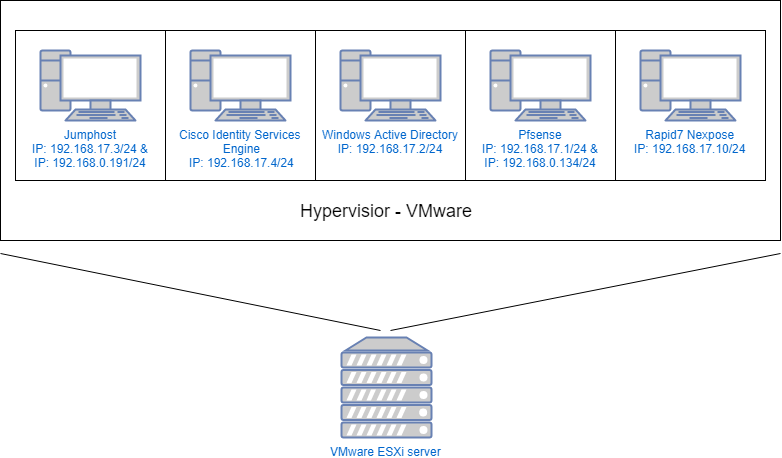
\includegraphics[height=0.3\textheight]{servervm.png}
	\caption{Virtuele machines in VMware ESXi server}
	\label{fig:vms}
\end{figure}

\newpage
Door de configuratie van deze IP instellingen, is de VMware ESXi server toeganglijk via de webbrowser. Virtuele machines kunnen via de webbrowser beheerd, verwijderd en gecreëerd worden. Daarnaast werd de hard disk drive ingesteld met een RAID controller. RAID, een afkoring voor Redundant array of independent disks is een dataopslagtechnologie waarbij meerdere harde schijven gecombineerd worden tot één of meer logische virtuele opslageenheden. Dit heeft als doel om de veiligheid, snelheid en de capaciteit te kunnen vergroten. Hierbij is op de VMware ESXi RAID 10 geconfigueerd. RAID 10 is een hybride combinatie tussen RAID 1 en RAID 0. Waarbij men de snelheid van striping met de veiligheid van mirroring combineert. 
\newline
\newline
Dit is de veiligste en snelste methode maar ook de duurste. Het is een dure methode omdat er gebruik wordt gemaakt van RAID 1, dus voor iedere 1TB aan opslagruimte is er ook 1TB aan mirror ruimte nodig, in combinatie met RAID 0 waardoor er veel fysieke harde schijven nodig zijn. In figuur \ref{fig:Raid10} wordt een voorbeeld van een RAID 10 schema weergegeven.

\begin{figure}[H]
	\centering
	\includegraphics[height=0.25\textheight]{Raid10.png}
	\caption{Voorbeeld configuratieschema RAID 10 (\cite{Raid10}).}
	\label{fig:Raid10}
\end{figure}

Vervolgens zijn er in de VMware ESXi server opstelling drie van de vier fysieke ethernet adapters gebruikt. Deze adapters zijn op hun beurt verbonden met een virtuele switch. Elk van de fysieke adapters heeft een andere functie die weergegeven zijn in de onderstaande lijst. 

\begin{itemize}
	\item vmnic0,is de fysieke adapter die verbonden is met de virtuele switch, genaamd 'VSwitch0'.
	\item vmnic2,is de fysieke adapter die verbonden is met de virtuele switch, genaamd 'Sub\textunderscore switch'.
	\item vmnic3,is de fysieke adapter die verbonden is met de virtuele switch, genaamd 'Cisco \textunderscore switch'.
\end{itemize}

\newpage
\subsubsection{Virtuele switches}
\subsubitem{\bf VSwitch0}
\newline
De 'VSwitch0' is een virtuele switch die voorzien is om de VMware ESXi server te contacteren via de webbrowser. Op figuur \ref{fig:Vswitch0} ziet men dat de 'VSwitch0' is ingesteld met vlan id 0, dat geen vlan identificatie voorziet. 
\newline
\newline
Data passeert deze interface wanneer gebruikers surfen naar "https://192.168.0.183". Vervolgens passeert de data langs de fysieke poort vmnic0 die data doorgeeft aan de VSwitch0. Wanneer data terecht komt op de VSwitch0, stuurt hij op zijn beurt de data door naar de VMKernel poort.

\begin{figure}[H]
	\centering
	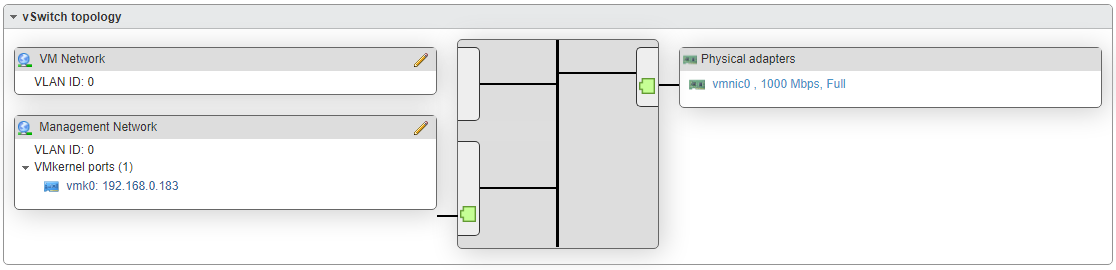
\includegraphics[width=0.7\textwidth]{VSwitch0.png}
	\caption{Topologie van de 'VSwitch0'}
	\label{fig:Vswitch0}
\end{figure}

\subsubitem{\bf Sub\textunderscore switch}
\newline
Op figuur \ref{fig:subswitch} ziet men dat de 'Sub\textunderscore switch' een virtuele switch is die gebruikt wordt voor WAN interface van de Pfsense. De Wide Area Network interface voorziet data overdracht van het thuisnetwerk naar het afgezonderd LAN netwerk. Hierdoor is connectie met het afgezonderd netwerk mogelijk via deze interface. Bovendien wordt deze virtuele switch ook gebruikt door de jumphost om remote desktop protocol connecties te maken met de virtuele machines binnen het afgezonderd LAN netwerk. 

\begin{figure}[H]
	\centering
	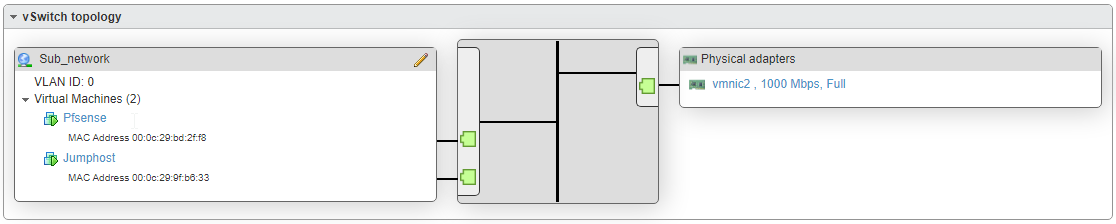
\includegraphics[width=0.7\textwidth]{Subswitch.png}
	\caption{Topologie van de 'Sub\textunderscore switch'}
	\label{fig:subswitch}
\end{figure}
\newpage
\subsubitem{\bf Cisco\textunderscore switch}
\newline
Ten slot is er de 'Cisco\textunderscore switch' die gebruikt wordt om connectie te maken met alle apparaten achterliggend de fysieke Cisco switch. Wanneer eind apparaten met de Cisco switch verbinden, dan zal de data passeren via de 'Cisco\textunderscore switch'. Bovendien is op figuur \ref{fig:Ciscoswitch} te zien dat alle virtuele machines zich in deze omgeving bevinden. Dit zorgt er voor dat de Cisco\textunderscore switch ingesteld is met vlan id 10, waarbij enkel data vanuit vlan 10 wordt doorgestuurd naar de voorziene eind apparaten.

\begin{figure}[H]
	\centering
	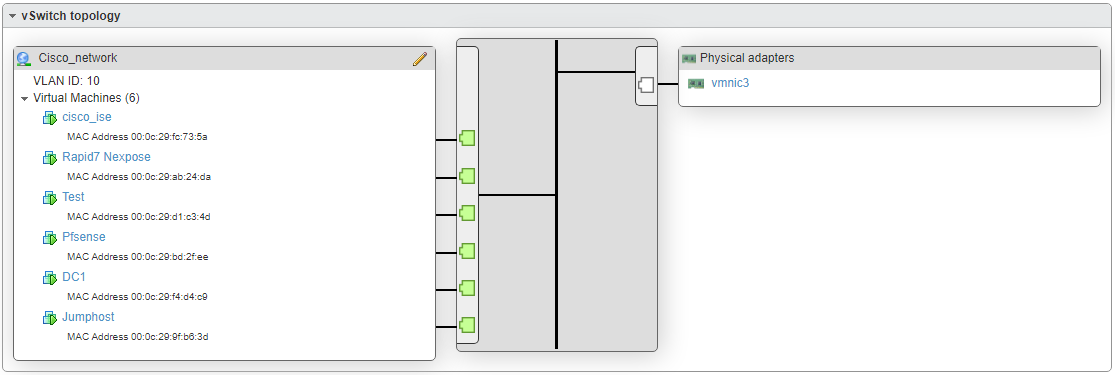
\includegraphics[width=0.7\textwidth]{CiscoSwitch_vmware.png}
	\caption{Topologie van de 'Cisco\textunderscore switch'}
	\label{fig:Ciscoswitch}
\end{figure}

\subsubsection{Server ESXi specificaties}
De VMware ESXi server is van het merk International Business Machines Corporation, gekend als IBM. Deze server werd oorsprongelijk gebruikt in de productie omgeving van Axians, maar wordt sinds kort als test server gebruikt. In figuur \ref{fig:VmwareSer} ziet men een afbeelding van de IBM ESXi server.
\newline
\newline
Het model van de VMware ESXi server is ‘System x3350 M3’ dat gekend staat binnen Axians als ‘de oude shr-esx-04 server’. De IBM ‘System x3350 M3’ bevat volgende specificaties:

\begin{itemize}
	\item Vormfactor: 1U Rack
	\item Processor:
	\begin{itemize}
		\item Proccessorsnelheid: 2.53GHz
		\item Processor: 6-core processor
	\end{itemize}
	\item Geheugen:
	\begin{itemize}
		\item Intern geheugen: 240 GB Random Access Memory
		\item Intern geheugentype: Double Data Rate 3 Synchronous Dynamic Random-Access Memory, gekend als DDR3 SDRAM
	\end{itemize}
	\item Opslag:
	\begin{itemize}
		\item Maximum aantal schrijven: 8 Slots
		\item Opslag: 4 Terabyte HHD 7500 RPM
	\end{itemize}
	\item Netwerk
	\begin{itemize}
		\item Ethernet interface type: Gigabit Ethernet
		\item Aantal ethernet poorten: 4 
	\end{itemize}
\end{itemize}

\begin{figure}[H]
	\centering
	\includegraphics[width=0.5\textwidth]{serveresxi.png}
	\caption{Foto van de ESXi VMware server}
	\label{fig:VmwareSer}
\end{figure}

\subsection{Cisco switch}
Naast de VMware ESXi server, bestaat de Cisco Identity Services Engine omgeving ook uit een Cisco switch. Dankzij een aantal configuraties op de Cisco switch kan de Cisco Identity Services Engine virtuele machine communiceren met de fysieke switch. Deze noodzakelijke configuraties speelden een belangrijke rol in de configuratie van de 'Port-based network access control' use case. 
\newline
\newline
Door een aantal basis configuraties op deze switch uit te voeren wordt communicatie tussen het afgezonderd netwerk en de eind apparaten die zich achter de Cisco switch bevinden ook mogelijk. Deze informatie is terug te vinden in de sectie \ref{sec:config}.

\subsubsection{Configuratie}
\label{sec:config}
Als eerst zijn een aantal commando's uitgevoerd die het netwerk apparaat beveiligen met een secret, line passwords en password encryption om inbreuk tegen te gaan. Vervolgens werd Gigabit Ethernet 0/1 geconfigureerd met de gepaste trunk settings om de gobale communicatie mogelijk te maken. Een trunk configuratie maakt data overdracht van de verschillende vlan's mogelijk. Volgende twee trunk commando's zijn hiervoor uitvoerd: 

\begin{itemize}
	\item switchport mode trunk
	\item switchport trunk allow vlan 10 
\end{itemize}

Gigabit Ethernet 0/1 werd rechtsverbonden met één van de interfaces op de VMware ESXi server, waarbij de virtuele switch ingesteld werd met vlan id 0 dat gelijk staan aan geen vlan identificatie. Vervolgens werd
op de Cisco switch vlan 10 gecreeërd met ip adres '192.168.17.5' en met subnet mask '255.255.255.0'. Vermits de interface Gigabit Ethernet 0/1 geconfigureerd is om verbinding te maken met de VMware ESXi server, zijn de overige interfaces bedoeld voor de communicatie met de eind apparaten. 
\newline
\newline
Om de 'Port-based network access control' use case te implementeren, werd een nieuw AAA model ingesteld. Dit AAA model werd vervolgens geïnitialiseerd met een radius server die gelijk staat aan het Internet Protocol adres van Cisco Identity Services Engine. Ten slotte werd de dot1x aaa authentication methode met zijn standaard netwerk groep mee configureerd. 
\newline
\newline
Om de configuraties van de Cisco switch te beëindeigen, werd dot1x system-auth-control vastgelegd en werden alle poorten voorzien van de nodige 'Port-based access control' configuraties. Figuur \ref{fig:RunningConfig} toont de running config van de Switch Cisco, daarnaast zijn alle nodige commando's in onderstaande lijst ook weergegeven.
\begin{itemize}
	\item \#enable
	\item \#config t
	\item (config)\#aaa new-model
	\item (config)\#aaa group server radius ISE
	\item (config-sg-radius)\#server-private 192.168.17.4 key Admin2020
	\item (config-sg-radius)\#exit
	\item (config)\#aaa authentication dot1x
	\item (config)\#aaa authorization network default group ISE
	\item (config)\#dot1x system-auth-control
	\item (config)\#interface range gig0/2-12
	\item (config-if-range)\#switchport mode access
	\item (config-if-range)\#switchmode access vlan 10
	\item (config-if-range)\#authentication host-mode multi-host
	\item (config-if-range)\#authentication port-control auto
	\item (config-if-range)\#dot1x pae auth
	\item (config-if-range)\#end
\end{itemize}

\begin{figure}[H]
	\centering
	\subfloat{{\includegraphics[width=3cm]{Switch_config1.png} }}%
	\qquad
	\subfloat{{\includegraphics[width=3cm]{Switch_config2.png} }}%
	\qquad
	\subfloat{{\includegraphics[width=3cm]{Switch_config3.png} }}%
	\caption{Running config van de Cisco switch}%
	\label{fig:RunningConfig}%
\end{figure}
Verder zijn 1G cat5e ethernet kabels gebruikt om de hardware componenten met elkaar te laten communiceren. De Unshielded Twisted Pair Ethernet kabels halen snelheden tot 1000 Mbit/s met een doorvoersnelheid van 100mhz. Wat geschikt is voor dit afgezonderd netwerk.

\subsubsection{Cisco switch specificaties}
De Cisco switch behoord tot de ‘Catalyst 2960-CX’ series die nu gekend staat binnen Axians als de ‘Demo switch’. Hierbij vindt men in onderstaande lijst de specificaties van de Cisco Catalyst 2960-CX serie switch:

\begin{itemize}
	\item Power over Ethernet:
	\begin{itemize}
		\item Ondersteunend: Ja
		\item Standaard: 802.3at (PoE+)
	\end{itemize}
	\item Netwerk:
	\begin{itemize}
		\item 8 Gigabit Ethernet aansluitingen
		\item 2 Gigabit Ethernet Copper uplinks
		\item 2 Gigabit Ethernet Small form-factor pluggable uplinks, gekend als SFP
	\end{itemize}
	\item Besturingsysteem/software:
	\begin{itemize}
		\item OS: Cisco IOS
    \end{itemize}
\end{itemize}


\subsection{Virtuele machines}
\subsubsection{Cisco Identity Services Engine}
De eerste virtuele machine waarop dieper wordt op ingegaan is Cisco Identity Services Engine. Deze virtuele machine zal zich verdiepen in de use cases: 'Port-based network access control', 'Policy-based network access control' en 'Thread-centric network access control'. Daarvoor zijn een aantal configuraties uitgevoerd op de virtuele machine van Cisco Identity Services Engine om een antwoord te geven het onderzoek. Hieronder worden de configuraties opgesplitst per use cases, waarbij de use cases vaak in de praktijk worden gecombineerd. De resultaten van de Cisco Identity Services Engine configuraties vindt men terug in Hoofdstuk \ref{ch:Resultaten}.
\newline
\newline
Alvorens men dieper ingaat op de use cases werd Cisco Identity Services Engine toegevoegd aan het Active Directory Domein. Figuren \ref{fig:AD_Cisco1} en \ref{fig:AD_Cisco2} tonen aan dat de virtuele machine van Cisco Identity Services Engine probleemloos toegevoegd is aan het domein 'Bachelorproef.com'. Dit toont aan dat Cisco Identity Services Engine eenvoudig geïntegreerd kan worden met een domein, waarbij in de toekomst extra policy rules kunnen ingevoerd worden. Dit onderzoek focust zich op de bescherming van de vrije interfaces op de Cisco switch door een extra authenticatie methode te voorzien en dus niet op integratie van 'Port-based network access control' het gebruik Active Directory Domein users.

De installatie van Cisco Identity Services Engine werd mogelijk gemaakt door \cite{CiscoISE_InstallationGuide}.

\begin{figure}[H]
	\centering
	\includegraphics[width=0.9\textwidth]{AD_ise.png}
	\caption{Cisco ISE gelinkt met het AD domein}%
	\label{fig:AD_Cisco1}%
\end{figure}

\begin{figure}[H]
	\centering
	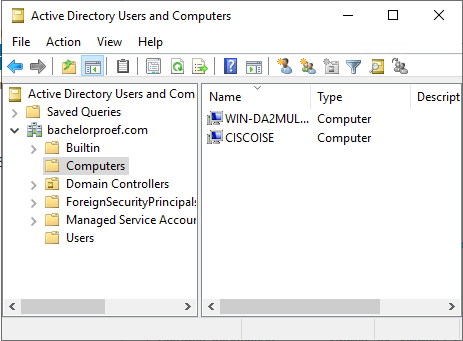
\includegraphics[width=0.7\textwidth]{ADComputers.png}
	\caption{Active Directory Users en Computers}
	\label{fig:AD_Cisco2}
\end{figure}
 \subsubitem{\textbf{Port- en Policy-based network access control }}
 \newline
 	Eerder werd vernoemd in sectie \ref{sec:config} dat voor implementatie van 'Port-based network access control' configuraties op de Cisco switch verplicht zijn. Op dit onderdeel van de sectie ligt de focus op de configuratie van de 'Port-based network access control' use case in de Cisco Identity Services Engine webbrowser. 
 	\newline
 	\newline
 	De Configuratie wordt gestart met de creatie van een aantal Cisco Identity Services Engine users in het 'Identity Management' tablad. In figuur \ref{fig:users} ziet men twee aangemaakte users waarbij user 'TestV2' zich in de groep 'Employees' bevindt en user 'Test' niet. Dit zal zich uiten wanneer een gebruiker zich aanmeldt met user 'Test' dan zal hij geen toegang krijgen tot het netwerk aan de hand van een policy rule.
 	
 	\begin{figure}[H]
 		\centering
 		\includegraphics[width=0.9\textwidth]{Port_users.png}
 		\caption{Cisco Identity Services Engine users}%
 		\label{fig:users}%
 	\end{figure}
 	
 	Vervolgens werd in het tablad 'Network Resources' de Cisco switch vastgelegd waardoor Cisco Identity Services Engine communicatie met het netwerk apparaat kan vaststellen. Figuur \ref{fig:ISESwitch} toont de configuratie voor deze communicatie. 
 	
 	 	\begin{figure}[H]
 		\centering
 		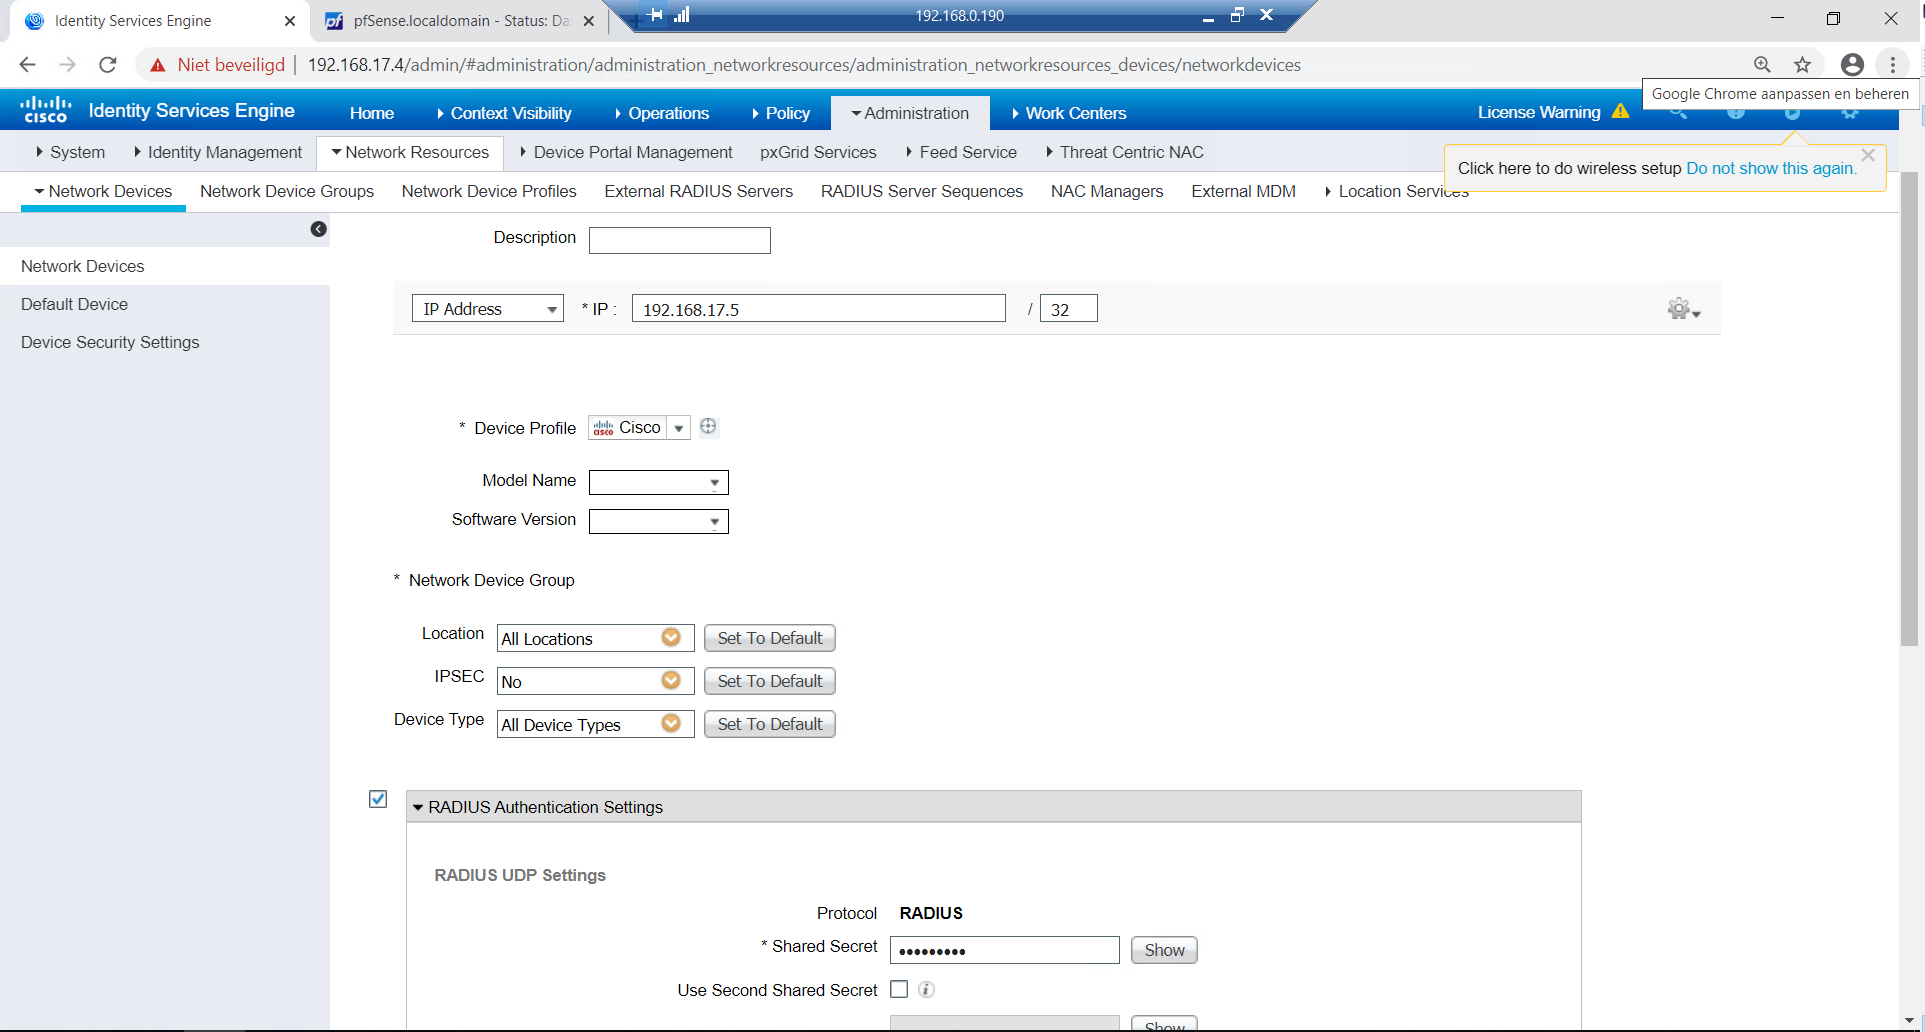
\includegraphics[width=0.7\textwidth]{ISESwitch.png}
 		\caption{Configuratie van de Cisco switch in ISE}%
 		\label{fig:ISESwitch}%
 		\end{figure}
 	
 	Ten slotte is een policy rule ingesteld waarbij gecontroleerd wordt of de gegevens overeenkomen met de instellingen van de policy rule. In dit geval laat de policy rule netwerk trafiek tot als de gebruiker de juiste identificatie gegevens ingeeft maar anderzijds ook wanneer de gebruiker zich in de groep 'Employees' bevindt. Op figuur \ref{label} is policy role weergegeven.
 	
	 	 \begin{figure}[H]
		\centering
		\includegraphics[width=0.7\textwidth]{PolicySet_Port.png}
		\caption{Configuratie van de 802.1x policy rule in ISE}%
		\label{fig:ISESwitch}%
		\end{figure}

 \subsubitem{\textbf{Thread-centri- en Policy-based network access control }}
  \newline
	!!!TO DO!!! Lorem ipsum dolor sit amet, consectetur adipiscing elit. Sed sed euismod velit, sed hendrerit justo. Praesent a hendrerit diam, ut imperdiet enim. In placerat nisl et commodo laoreet. Nullam convallis semper nibh nec cursus. Pellentesque a urna iaculis, eleifend turpis sit amet, varius velit. Nulla vitae est euismod, feugiat sem quis, fringilla nibh. Quisque ornare orci nisl, non pretium felis tempor id. Proin varius fermentum velit eu imperdiet. Praesent quis dolor at metus ornare dignissim sed finibus mauris. Maecenas pellentesque, ante ac vulputate dapibus, nisl nisi tristique libero, eu sollicitudin dolor est nec quam. Sed in lobortis sem. Phasellus nec diam eu magna lacinia tincidunt vitae in elit.
 
Verder werd systeem geïnstalleerd op een Red Hat Enterprise 7 distributie, waar vogende specificaties voor werd vrijgemaakt: 

\begin{itemize}
	\item Geheugen: 128 GB Random Access Memory
	\item Opslag: 512 GB
	\item CPU: 24 cores
	\item Netwerk adapter: Cisco\textunderscore netwerk
\end{itemize}

\subsubsection{Windows server 2019 datacenter}
Het gebruik van een Windows Server 2019 maakt de creatie van een Active Directory domein mogelijk. Een nieuwe forest werd hiervoor aangemaakt en de Windows Server 2019 werd meteeon ook gepromoveerd naar de domeincontroller binnen het 'bachelrorproef.com' netwerk.
\newline
\newline
Via Cisco Identity Service Engine kan men subset van domeinen selecteren vanuit de vertrouwde domeinen voor authenticatie en autorisatie. Deze subset van domeinen worden authenticatiedomeinen genoemd. Het definiëren van deze authenticatiedomeinen verbetert de beveiliging door bepaalde domeinen te blokkeren, waardoor de authenticatie van de gebruikers op deze domeinen wordt beperkt.
\newline
\newline
Zoals voorheen vermeld is integratie met Windows Server Active Directory en Cisco Identity Services Engine reeds mogelijk. Hierdoor kunnen bedrijven met Cisco Identity Services opteren om werknemers te laten inloggen op het netwerk met de 'Domain Users. Vaak wordt deze methode geïntegreerd met het 'wireless' aanmelden op netwerk door gebruik van de Active Domain Directory gegevens. Helaas beschikte dit afgezonderde netwerk niet over een wireless controller die dit mogelijk maakt. Cisco Identity Services voorziet hiervoor vooraf gedefinieerde regels.

Verder wordt het ‘Remote Desktop Protocol (RDP)’ in combinatie met het Internet Protocol (IP) adres gebruikt om de Windows machines te bereiken.
\newline
\newline
Om de Windows server 2019 datacenter te gebruiken werden volgende specificaties vrijgemaakt:

\begin{itemize}
	\item Geheugen: 16 GB Random Access Memory
	\item Opslag: 126 GB
	\item CPU: 20 cores
	\item Netwerk adapter: Cisco\textunderscore netwerk
\end{itemize}

Als laatstse werd de installatie van Windows Server 2019 datacenter mogelijk gemaakt door \cite{Win19_InstallationGuide}. 

\subsubsection{Pfsense}
De Pfsense virtuele machine verwijst naar de virtuele router waarbij één interface van de Pfsense gebruikt wordt als gateway voor alle vlan’s en van alle componenten die zich achter de Cisco switch bevinden. Vervolgens wordt de WAN interface van de Pfsense gebruikt om de data van en naar de Local Area Network interface te sturen. Hierdoor is communicatie vanuit het thuisnetwerk met het afgezonderd netwerk mogelijk.
\newline
\newline
De pfsense is enkel te contacteren binnen het afgezonderd netwerk door het ‘Hypertext Transfer Protocol (HTTP)’ te gebruiken. Met andere woorden kunnen enkel machines in het netwerk '192.168.17.0/24' de Pfsense interface bereiken door te surfen naar het ip adres: '192.168.17.1'. Op figuur \ref{fig:Pfsense} is te zien dat de home interface van de Pfsense te bereiken is via 'http://192.168.17.1/'.
\newline
\newline
Ten slotte werd dit systeem geïnstalleerd op een Free Berkeley Software Distribution, waar volgende specificaties zijn voor vrijgemaakt: 

\begin{itemize}
	\item Geheugen: 4 GB Random Access Memory
	\item Opslag: 25 GB
	\item CPU: 4 cores
	\item Netwerk adapter: Cisco\textunderscore netwerk
\end{itemize}
De installatie van Pfsense werd mogelijk gemaakt door \cite{Pfsense_InstallationGuide}.

\begin{figure}[H]
	\centering
	\includegraphics[width=0.7\textwidth]{PfsenseHome.png}
	\caption{Home interface Pfsense}
	\label{fig:Pfsense}
\end{figure}

\subsubsection{Jumphost}
Een jumphost is een tussenliggende host machine waarbij connectie naar een extern netwerk mogelijk is. Vervolgens kan een verbinding worden gemaakt met een andere host in het extern netwerk. Met andere woorden 'jumpt' men dus van het ene apparaat naar het andere om een extern netwerk te bereiken. 
\newline
\newline
Dit werd in de Cisco Identity Services Engine omgeving ook gebruikt waarbij een eind apparaat in het thuisnetwerk verbinding maakt met de Jumphost via Remote Desktop Protocol om zo eind apparaten in het afgezonderd netwerk te contacteren. Hierbij zijn volgende instellingen gebruikt:  

\begin{itemize}
	\item Geheugen: 16 GB Random Access Memory
	\item Opslag: 126 GB
	\item CPU: 20 cores
	\item Netwerk adapter 1: Cisco\textunderscore netwerk
	\item Netwerk adapter 2: Sub\textunderscore netwerk
\end{itemize}

De installatie van Pfsense werd mogelijk gemaakt door \cite{Pfsense_InstallationGuide}.

\subsection{Begrippen}
\subsubitem{\textbf{Telenet Access Point}} is een draadloze server die gegevens verzendt via radio golven in middel van een antenne. Deze gegevens worden ontvangen via het bedrage UTP netwerk waarbij deze “server” is op aan gesloten.
\subsubitem{\textbf{Telenet Modem}} is een toestel die informatie van uw internetprovider ontvangt via een telefoonlijn, glasvezelkabel of coaxkabel in de woning en converteert dit naar een digitaal signaal.
\subsubitem{\textbf{Coax kabel}} is een twee polige kabel die instaat voor het overdragen van beeld en geluid. Deze signalen treden gemakkelijker binnen, waarbij het signaal op korte afstanden snel zwak wordt. 
\subsubitem{\textbf{Virtual local area network}} is een type virtueel network dat gerealiseerd wordt op de datalinklaag. Dit bestaat uit een groep eindstations en switches die logisch gezien één enkel gemeenschappelijk local area network (LAN) vormen.
\subsubitem{\textbf{Local Area Network}} is een computernetwerk dat een relatief klein gebied beslaat. Meestal is een LAN beperkt tot een kamer, een gebouw of een groep gebouwen, waarbij een LAN kan via telefoonlijnen en radiogolven over elke afstand met andere LAN's kan communiceren.
\subsubitem{\textbf{Wide Area Network}}  is een netwerk van apparaten, een verzameling van local area networks, die via draadloze of bekabelde communicatielijnen met elkaar verbonden zijn.

\section{Cisco Identity Services Engine enquête}
\label{sec:enquête}
Om een link te leggen met de resultaten van de uitgevoerde testen, werd een enquête of een formulier opstelt. Deze enquête is als onderliggende basis gebruikt bij de analyse van de resultaten die verkregen werden door de fysieke testen. Zoals in vorige hoofdstukken vermeld, is deze enquête een opiniepeiling. Waarbij een aantal vragen gesteld zijn aan personen die reeds gekend zijn met Cisco Identity Services Engine. Hierdoor is de doelgroep van deze enquête beperkt tot de Cisco Identity Services Engine specialisten.
\newline
\newline
Deze enquête is publiekelijk gemaakt via LinkedIn en via E-mail. Linkedin is een online sociaal netwerk dat is opgericht voor Vakmensen, die ongeveer 610 miljoen geregistreerden telt. Omdat deze enquête publiekelijk werd gemaakt op \cite{LinkedIn}, bevat dit formulier een aantal ‘failsave’ vragen. Deze ‘failsave’ vragen zijn bedoelt wanneer niet Cisco Identity Services Engine specialisten de enquête proberen in te vullen. Met als gevolg dat de kans op onjuiste ingevuld antwoorden verkleind werd.
\newline
\newline
Dit formulier of enquête werd mogelijk gemaakt door Microsoft en Hogeschool Gent. Elke student heeft recht op een gelicentieerd Office 365 pakket gedurende zijn opleidingstraject. Het programma in kwestie noemt men \cite{MicrosoftForms} dat inbegrepen is in het Microsoft Office 365 pakket.
\newline
\newline
Een overzicht van de vragen die gesteld werden tijdens de enquête is terug te vinden in \ref{ch:Resultaten_enquête}. Bij elke vraag is steeds een klein woordje uitleg gegeven. Idem zoals de mogelijke antwoorden en eventuele doorverwijzingen naar andere vragen.



 \chapter{\IfLanguageName{dutch}{Resultaten}{Resultaten}}
\label{ch:Resultaten}
In dit hoofdstuk zullen de resultaten van de testen en de enquête verwerkt worden om tot een antwoord te komen van dit onderzoek. Hierbij zijn de resultaten van de Cisco Identity Services Engine omgeving opgedeeld in 'Port-based en Policy-based network access control' en 'Thread-Centric en Policy-based network access control '. Vervolgens zijn de enquête resultaten verwerkt met een aantal grafieken waarbij de resultaten terug te vinden zijn in Bijlage \ref{ch:Resultaten_enquête}. Meer informatie over de resultaten van de enquête vindt men in sectie \ref{sec:enqueteISe}.

\section{Cisco Identity Services Engine omgeving}
Zoals men ziet wordt Policy-based network access control steeds gecombineerd met Port-based en Thead-Centric network access control. Dit heeft als reden dat zowel Port-based, als voor Thread-Centric network access control, policy rules zijn toegepast. In elk van deze subsecties worden de resultaten van voor de implemenatie van de Cisco Identity Services Engine use cases  en na de implemenatie van deze use case toegelicht. Op die manier kan in hoofdstuk \ref{ch:conclusie} een conclusie gemaakt worden die een duidelijk antwoord biedt op dit onderzoek.  
\subsection{Port-based en Policy-based network access control}
Wanneer de use cases 'Port-based en Policy-based network access control' niet worden toegepast, dan kunnen gebruikers zich aansluiten op het netwerk zonder enige beveiliging. Dit is natuurlijk enkel mogelijk wanneer alle interfaces op het netwerk apparaat ingesteld zijn met het correcte vlan id. Anderzijds is het duidelijk dat eind apparaten zich eenvoudiger kunnen aansluiten op het netwerk zonder de implementatie van 'Port-based en Policy-based network access control' use cases.
Als men de resultaten van de implemenatie van 'Port-based en Policy-based network access control' erbij halen, dan ziet men een duidelijk verschil in beveiliging ten opzichte van een netwerk zonder de use cases. Dit verschil is duidelijk te merken wanneer een gebruiker zich probeert aan te melden op het netwerk via één van de interfaces op de fysieke Cisco switch. Het eind apparaat wijst zichzelf een ip-adres toe van de vorm 169.254.x.x dat geen enkel compartiment van het netwerk kan bereiken. 
\newline
\newline
Het is echter wanneer de 'Wired AutoConfig' services aanstaan dat men zich kan aanmelden op het netwerk door de volgende stappen uit te voeren: 
\begin{itemize}
	\item Open het configuratiescherm, en ga naar 'netwerk en internet'.
	\item Open vervolgens het 'netwerkcentrum'.
	\item Open 'Adapter instellingen wijzigen'.
	\item Open het 'properties' tablad, door een rechtermuisklik op de correcte "Ehternet adapter".
	\item Vervolgens verschijnt het tablad "Authenticatie".
	\item Open "Extra instellingen".
	\item Veranderd de 'authentication modus' naar 'gebruikers authenticatie'.
\end{itemize}

Als de eind gebruikers de juiste gebruikersnaam en wachtwoord ingeeft, wordt de gebruiker met zijn apparaat aangesloten op het netwerk. Belangrijk om te weten is dat er een policy rule zo ingesteld is dat alleen gebruikers van de groep 'Employees' toegang krijgen tot het netwerk. Het gebruik van de policy werd al eerder vernoemd in het hoofdstuk \ref{ch:Proof of concept}.
Figuur \ref{fig:Test_gebruiker} toont aan dat wanneer men wenst in te loggen met de gebruikersnaam 'Test' geen toegang krijgt tot het netwerk. Gebruiker 'Test' bevindt zich niet in de groep 'Employees' en zal dus als gevolg geen toegang krijgen tot het netwerk. Dankzij het gebruik van policy rules wordt de proef aangetoond dat policy rules ook de vruchten kan plukken op beveiliging.

\begin{figure}[H]
	\centering
	\subfloat{{\includegraphics[width=5.5cm]{Test_no_employee.png} }}%
	\qquad
	\subfloat{{\includegraphics[width=5.5cm]{Test_no_successed.png} }}%
	\newline
	\subfloat{{\includegraphics[width=11.5cm]{TestDenied.png} }}%
	\caption{Proef resultaat met een niet employee gebruiker}%
	\label{fig:Test_gebruiker}%
\end{figure}

Als men inlogt met een gebruiker die in de Cisco Identity Services Engine groep 'Employees' bevindt dan zal de gebruiker zonder problemen zich kunnen aansluiten op het netwerk. Dit wordt aangetoond in figuur \ref{fig:Test_gebruiker} waarbij een proef met de gebruiker 'TestV2' wordt uitgevoerd. Gebruiker 'TestV2' bevindt zich in groep 'Employees' waardoor het vanzelfsprekend is dat 'TestV2' met zijn eind apparaat met het netwerk kan verbinden. 

\begin{figure}[H]
	\centering
	\subfloat{{\includegraphics[width=6cm]{TestV2_Employee.png} }}%
	\qquad
	\subfloat{{\includegraphics[width=6cm]{TestV2_succeeded.png} }}%
	\newline
	\qquad
	\subfloat{{\includegraphics[width=12cm]{TestV2_succeeded_ISE.png} }}%
	\caption{Proef resultaat met een employee gebruiker}%
	\label{fig:Test_gebruiker}%
\end{figure}

Vervolgens werd bij de tweede proef een policy rule geïmplementeerd die de toegang naar het netwerk vanuit de Cisco switch blokkeert op specifieke weekdagen.  De proef zou moeten aantonen wanneer gebruiker 'X' zich op woensdag aansluit op het netwerk dan zou gebruiker 'X' met zijn eindapparaat geen toegang krijgen.
Op Figuur \ref{fig:Woensdag} is te zien dat gebruiker 'TestV4' met de 'Port-based network access control' use case zich probeert aan te sluiten op het netwerk. 

\begin{figure}[H]
	\centering
	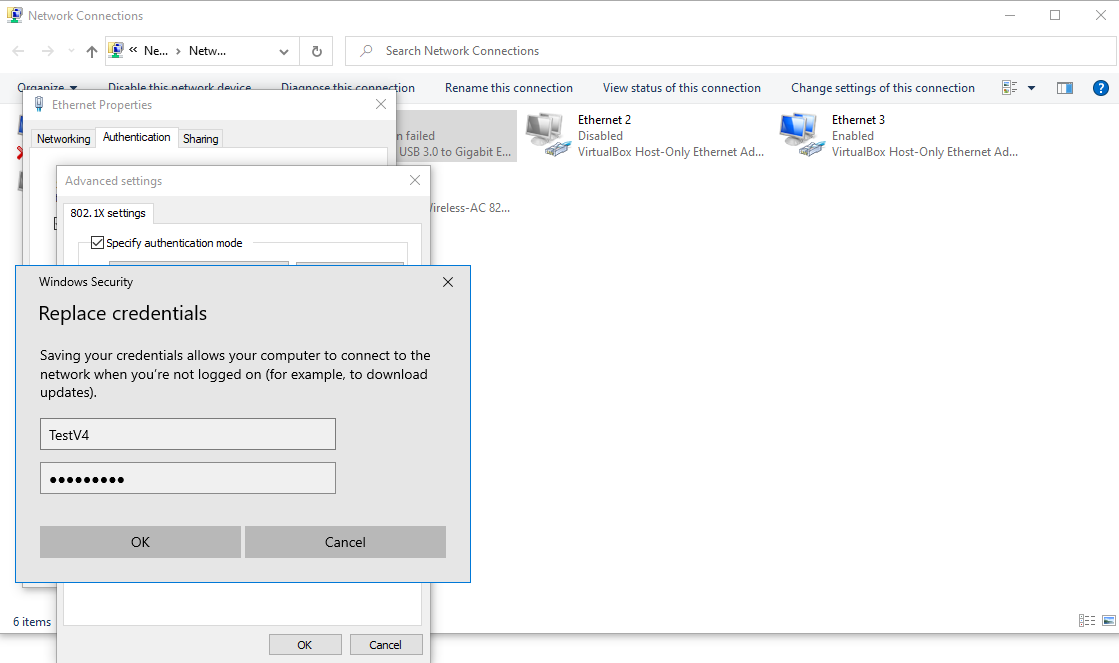
\includegraphics[height=0.20\textheight]{TestV4_Employee.png}
	\caption{Grafiek resultaat vraag 2}
	\label{fig:Woensdag}
\end{figure}

Het is al snel duidelijk dat Cisco Identity Services Engine toegang tot het netwerk blokkeert. Cisco Identity Services Engine registreert dat gebruiker 'TestV4' zich probeert aan te sluiten op het netwerk maar wordt vervolgens de toegang onmiddelijk ontnomen. Dit wordt aangetoond op figuur \ref{fig:failed} waarbij de toegang tot het netwerk voor gebruiker 'TestV4' geblokkeerd werd. 

\begin{figure}[H]
	\centering
	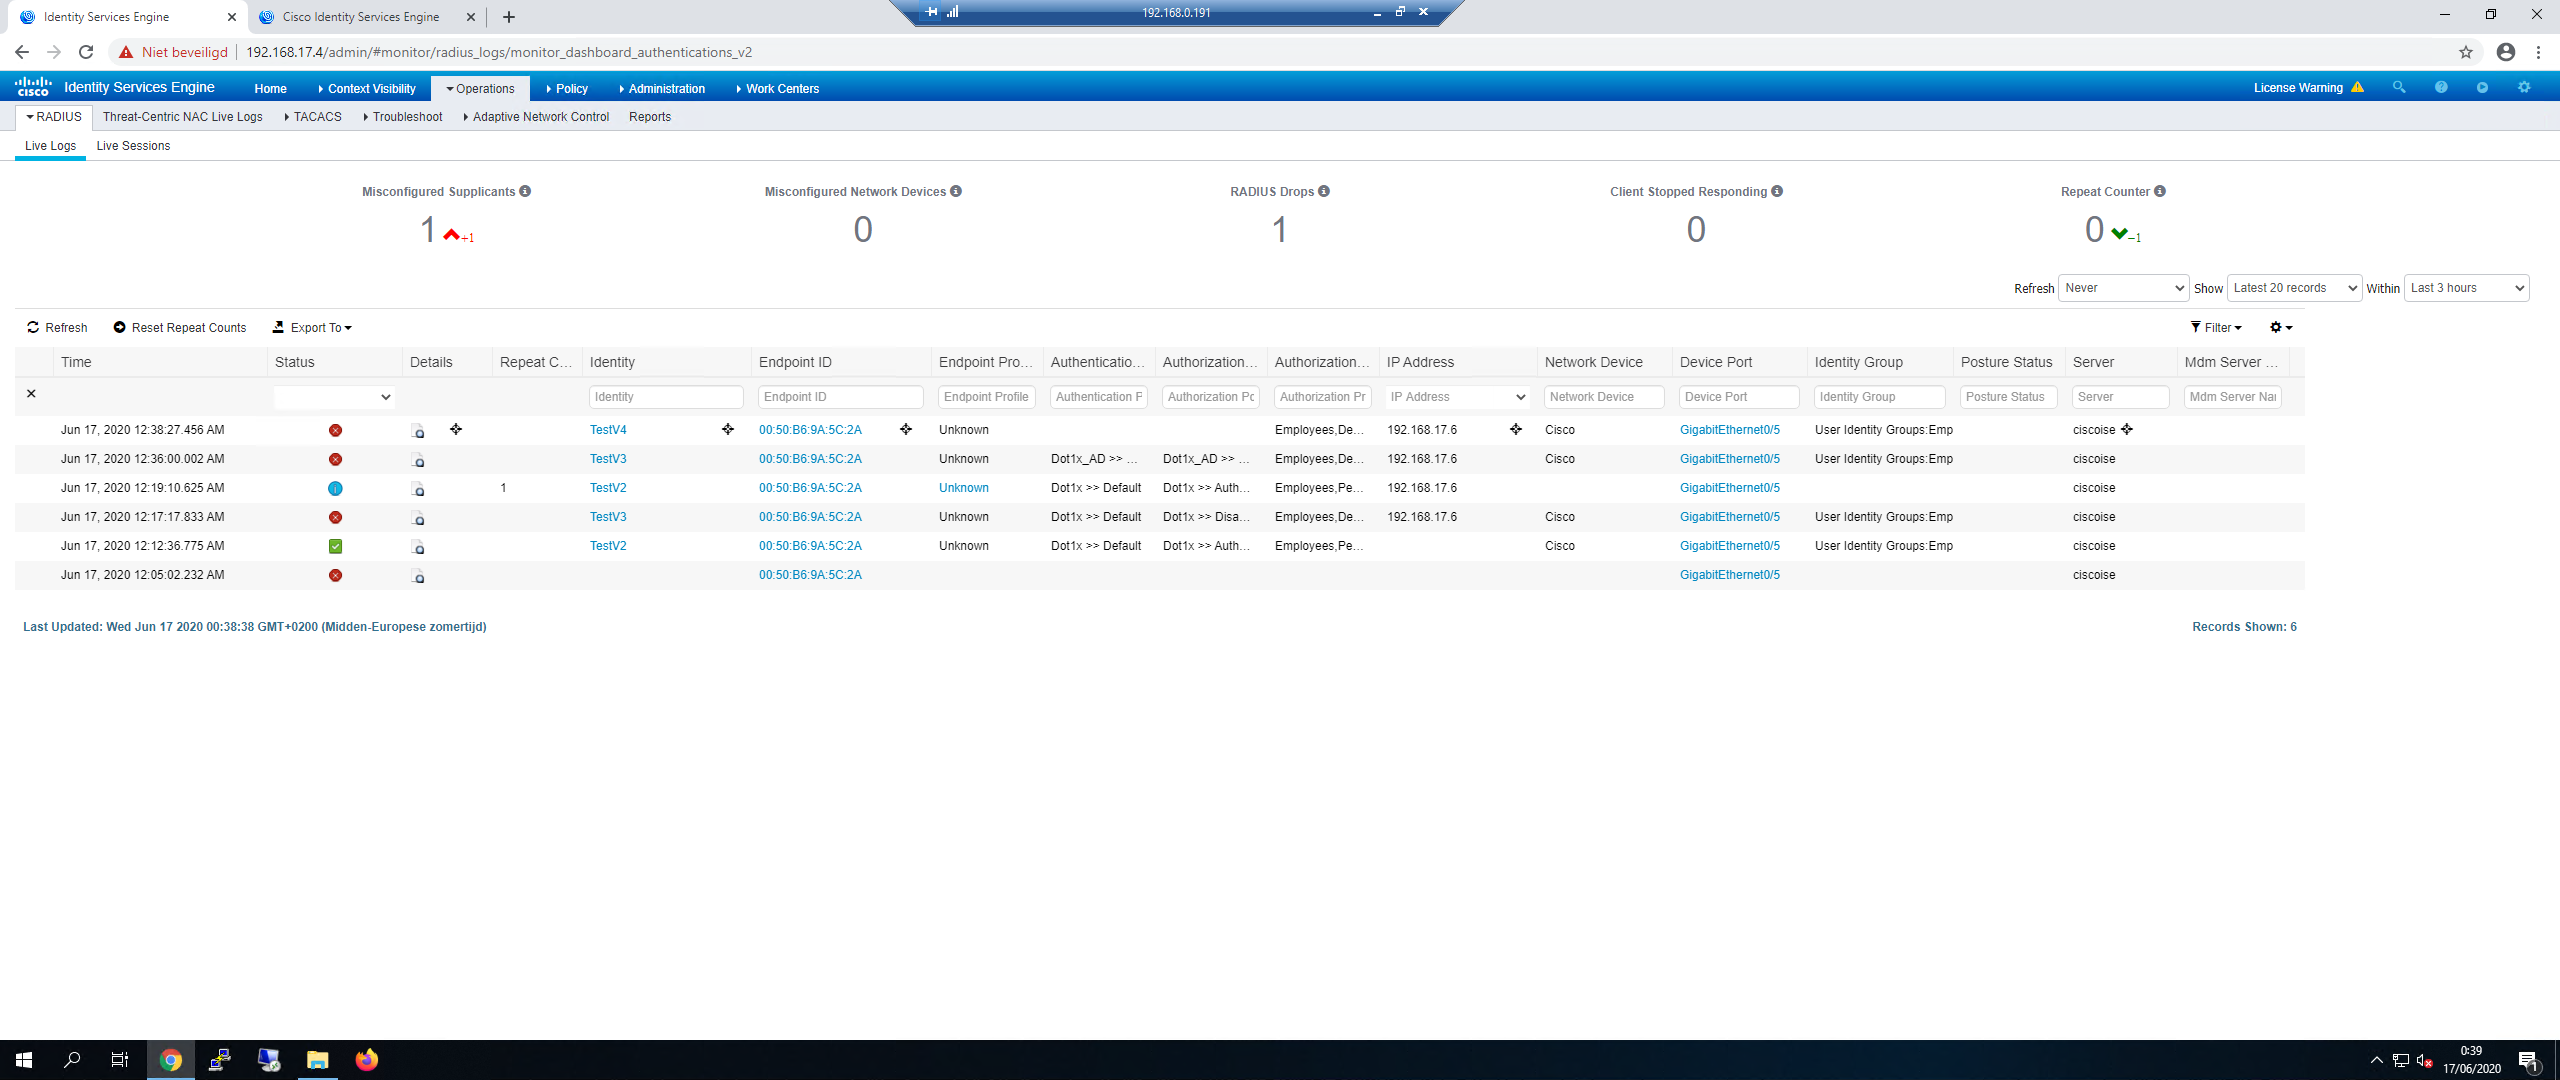
\includegraphics[height=0.20\textheight]{UsersFailed_Suc.png}
	\caption{Grafiek resultaat vraag 2}
	\label{fig:failed}
\end{figure}

Om aan te tonen dat gebruiker 'TestV4' het netwerk werd ontnomen door de 'Disable\textunderscore at\textunderscore weekend' policy rule kan men het rapport terug vinden in figuur \ref{fig:failed2}. Op deze figuur is te zien dat 'Disable\textunderscore at\textunderscore weekend' het desbetreffende Authorization policy rule was die werd uitgevoerd dat resulteerde in geen toegang tot het netwerk. 

\begin{figure}[H]
	\centering
	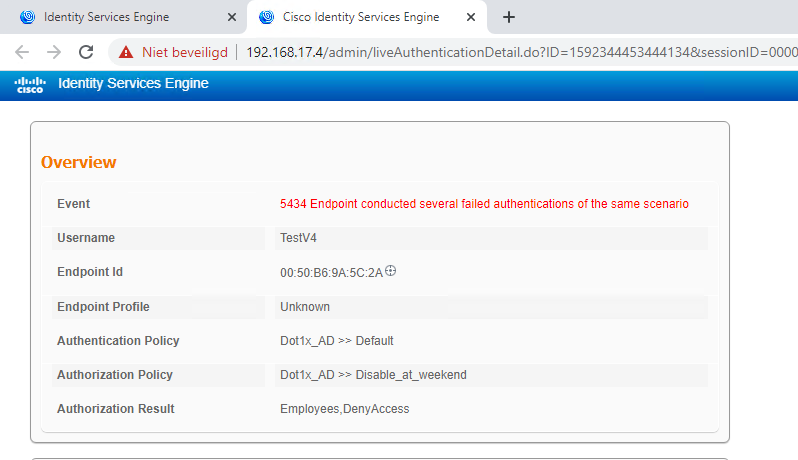
\includegraphics[height=0.20\textheight]{TestV4_failed.png}
	\caption{Grafiek resultaat vraag 2}
	\label{fig:failed2}
\end{figure}

Ten slotte toont figuur \ref{fig:ping} aan dat het eindapparaat na blokkade van het netwerk geen enkel component in het afgezonderd netwerk kan bereiken. Hiervoor werd het commando: 'Ping 192.168.17.1' uitgevoerd waarbij het eindapparaat de default gateway tracht te bereiken.

\begin{figure}[H]
	\centering
	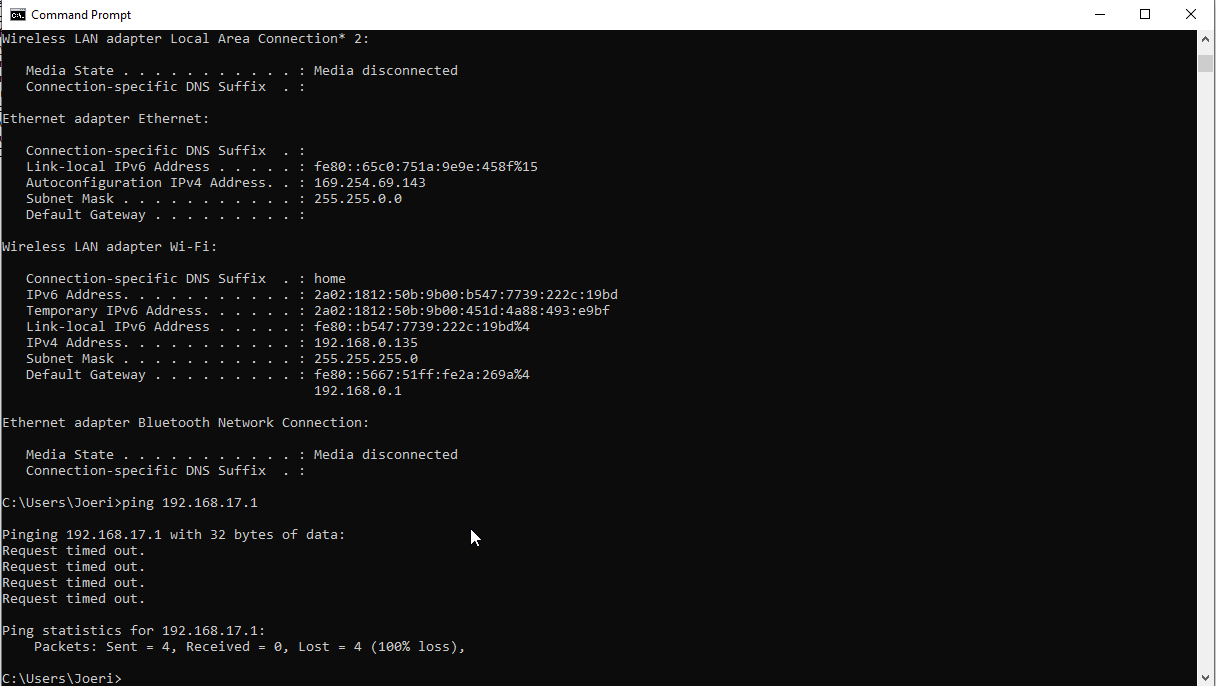
\includegraphics[height=0.20\textheight]{PingTestV4_failed.png}
	\caption{Grafiek resultaat vraag 2}
	\label{fig:ping}
\end{figure}


Men bekomt door het gebruik van Cisco Idendity Services Engine en use cases 'Port-based en Policy-based network access control' een positieve resultaat. Hieruit kan men uit de resultaten van de proef afleiden dat 'Port-based en Policy-based network access control' het bedrijfsnetwerk zeker en vast veiliger maakt tegen criminelen die het netwerk willen binnentreden. Dit komt door de beschikbare interfaces. Werknemers zullen in het vervolg zich eerst moeten aanmelden met de Cisco Identity Services Engine gegevens alvorens men voor de eerste keer connectie wilt maken met het netwerk. Nadien blijven deze gegevens opgeslagen op het eind apparat. Zo kan men steeds probleemloos verbinden met het netwerk via de Ethernet kabel.

In de sectie \ref{sec:trepo} worden de resultaten van Tread-Centric en Policy-based network access control besproken. Voor meer uitleg over de volledige conclusie kan men terecht in Hoofdstuk \ref{ch:conclusie}.


\subsection{Tread-Centric en Policy-based network access control}
\label{sec:trepo}
	!!!TO DO!!! Lorem ipsum dolor sit amet, consectetur adipiscing elit. Sed sed euismod velit, sed hendrerit justo. Praesent a hendrerit diam, ut imperdiet enim. In placerat nisl et commodo laoreet. Nullam convallis semper nibh nec cursus. Pellentesque a urna iaculis, eleifend turpis sit amet, varius velit. Nulla vitae est euismod, feugiat sem quis, fringilla nibh. Quisque ornare orci nisl, non pretium felis tempor id. Proin varius fermentum velit eu imperdiet. Praesent quis dolor at metus ornare dignissim sed finibus mauris. Maecenas pellentesque, ante ac vulputate dapibus, nisl nisi tristique libero, eu sollicitudin dolor est nec quam. Sed in lobortis sem. Phasellus nec diam eu magna lacinia tincidunt vitae in elit.

\section{Cisco Identity Services Engine enquête}
\label{sec:enqueteISe}
In deze sectie worden de resultaten van de enquête globaal besproken. Indien men meer informatie wenst over de resultaten per vraag kan men Bijlage \ref{ch:Resultaten_enquête} raadplegen.
\newline
\newline
Bovenal mag men zeker tevreden zijn met de responsen van de enquête daarnevens kent de enquête 14 responsen op 2 weken tijd. Helaas beschikt men niet over het grote netwerk om de responsen van de enquête te doen verhogen. Een groter aantal responsen zou resulteren in een veel nauwkeuriger resultaat.  
\newline
\newline
78.6\% van de geënquêteerden is gekend met het Cisco Identity Services Engine product. De overige 21.4\% is niet gekend met het Cisco Identity Services Engine product en is dus niet vertrouwd met network access control technolgieën. Bij gevolg weten de geënquêteerden niet welk alternatief in hun omgeving wordt toegepast waardoor vraag 4 en 5 geen antwooren kent. Van de personen die gekend zijn met Cisco Identity Services Engine is bij iedereen het product geïmplementeerd in hun bedrijfsomgeving. Wanneer de vraag werd gesteld waar ze voor het eerst Cisco Identity Services Engine hebben gehoord. Dan reageert 71.4\% van de responsen met het antwoord 'In de organisatie'. Het overschot van de responsen is gelijk verdeelt tussen 'Tijdens een webinair', ‘Tijdens een opleiding' en 'Op het internet'. Figuur \ref{fig:vraag2} kan hiervoor geraadpleegd worden. 
\begin{figure}[H]
	\centering
	\includegraphics[height=0.20\textheight]{Vraag2.png}
	\caption{Grafiek resultaat vraag 2}
	\label{fig:vraag2}
\end{figure}
De resultaten waarbij men de rede waarom men Cisco Identity Services Engine heeft gekozen in een hun bedrijfsomgeving moest ingeven, ligt gelijkmatig verspreid. Wat wel duidelijk is dat het antwoord 'Omwille van de betere beheerbaarheid van eind apparaten.' een hoger percentage kent dan de overige antwoorden. Dit ziet met ook in grafiek \ref{fig:graf6} duidelijk terug.
\begin{figure}[H]
	\centering
	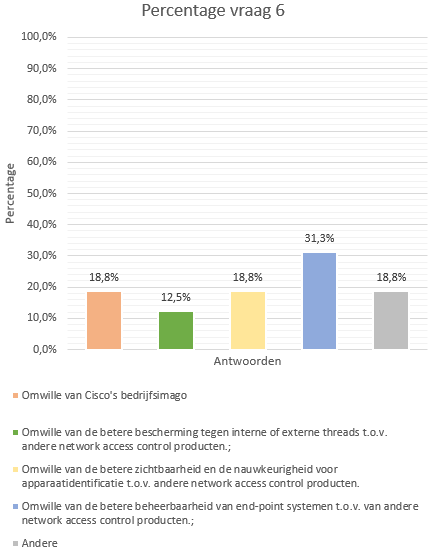
\includegraphics[width=0.50\textwidth]{Vraag6.png}
	\caption{Grafiek resultaat vraag 6}
	\label{fig:graf6}
\end{figure}
Uit vraag 7 kan afgeleidt worden dat 'Identiteits- en toegangsbeer','beleidshandhaving', 'Functionaliteit' en 'Uitbreidbaarheid' de belangrijkste kermerken zijn voor de keuze van het type network access control. Figuur \ref{fig:vraag7} toont daarbij de resultaten terug waarbij zeer duidelijk te zien is dat de vorige benoemde resultaten een zeer belangrijke rol spelen in de keuze van het network access control product. 

\begin{figure}[H]
	\centering
	\includegraphics[height=0.30\textheight]{Vraag7.png}
	\caption{Grafiek resultaat vraag 7}
	\label{fig:vraag7}
\end{figure}

Voor de volgende vraag kan men concluderen dat de veranderingen die bedrijven ondervinden na implementatie van Cisco Identity Services Engine verschillende zijn van responder tot responder. Globaal gezien komt dit wel overeen met elkaar dat Cisco Identity Services Engine de zichtbaar van eind apparaten op het netwerk verhogen. Een verbetering in troubleshooting is ook een van de veranderingen die de geënquêteerden ondervonden. Meer informatie over deze antwoorden is terug te vinden in bijlage \ref{tab:vraag8}. Vervolgens vindt 54.5\% van de geënquêteerden dat Cisco Identity Services Engine het product gelijkaardig vindt ten opzichte van andere network access control. Het is echter zo dat 9.1\% van de responders vindt dat Cisco Identity Services Engine slechter is dan zijn concurrenten. De rede achter dit kan helaas niet onbeantwoord worden. Verder bevat 36.4\% van de antwoorden het antwoord 'Beter'. Figuur \ref{fig:vraag9} geeft deze verwoording visueel terug. 

\begin{figure}[H]
	\centering
	\includegraphics[height=0.30\textheight]{Vraag9.png}
	\caption{Grafiek resultaat vraag 9}
	\label{fig:vraag9}
\end{figure}

De resultaten van de vraag: 'Wat zijn volgens u de meeste voorkomende modules of use cases van Cisco Identity Services Engine?', zijn in figuur \label{fig:vraag10} terug te vinden. Hierbij is duidelijk te zien dat merendeel van de geënquêteerden vindt dat 'Identity-based network access control' de belangrijkste use case van Cisco Identity Services Engine. Vervolgens komt het 'Policy-based network access control' dat daarna gevolgd wordt door het 'Thread-Centric network access control'. Hieruit kan men concluderen dat de proef een onderzoek uitvoert naar de bijna belangrijkste use cases. Het is toch verbazend dat slecht 7.7\% van de personen koos voor een 'Port-based network access control' use case. 

\begin{figure}[H]
	\centering
	\includegraphics[height=0.30\textheight]{Vraag10.png}
	\caption{Grafiek resultaat vraag 10}
\end{figure}

Daarnaast blijkt ook dat 54.5\% zegt dat Cisco Identity Services Engine nadelen kent binnen een netwerk. Deze nadelen uiten zich als 'Certificate updates require nac to shut down', 'het netwerk is afhankelijk van de nac oplossing', 'Instabiliteit van connecties met sommige systemen', enzovoort. Verder werd er ook heel wat voordelen opgesomd door de vakspecalisten die weergegeven zijn in \ref{tab:vraag11}. Alle antwoorden zijn terug te vinden in bijlage \ref{tab:vraag13}.
\newline
\newline
Uit vragen 14 en 15 is gebleken dat Cisco Identity Services Engine een logische keuze is ten opzichte van andere network access control producten. De resultaten van vraag 14 is 90.9\% voor het antwoord 'Ja' en 9.1\% met het antwoord 'Neen'. Vraag 15 toont aan dat 100\% van de vakspecalisten vindt dat een network access control product noodzakelijk is in een bedrijfsomgeving. Hieruit kan men concluderen dat een network access control zoals Cisco Identity Services Engine voor velen een echte must is.
Hierbij zijn de Antwoordenterug te vinden in bijlage \ref{tab:vraag13}. Verder werd er ook heel wat voordelen opgesomd door de vakspecalisten die weergegeven zijn in \ref{tab:vraag11}.
\newline
\newline
18.2\% van de personen die de enquête invulden vinden dat er functionaliteiten ontbreken in Cisco Identity Services Engine. De betreffende missende functionaliteiten zijn 'Industriële gerichtheid, incl. goede support voor staticshe ip adressen.' en 'Saml integratie in een samenwerking met Azure AD en Captive portal voor byod.’.


Tot slot kreeg Cisco Identity Services Engine een gemiddelde beoordeling van 3.91 op 5 waarbij 90.9\% van de geënquêteerden dit product zou aanbevelen aan anderen.




%%=============================================================================
%% Conclusie
%%=============================================================================

\chapter{Conclusie}
\label{ch:conclusie}

In dit onderzoek wordt een antwoord gegeven op de onderzoeksvraag 'Hoe kunnen we een evoluerend bedrijfsnetwerk beter gaan beveiligen door het gebruik van Cisco Identity Services Engine?' Hiervoor is er een studie uitgevoerd waarbij verschillende proeven zijn uitgewerkt die de nood van de Cisco Identity Services Engine use cases naar boven haalt. Vervolgens is de studie aangevuld met een enquête die een opiniepeiling vormt over Cisco Identity Services Engine en zijn use cases.
\newline
\newline
De resultaten van de 'Port-based en Policy-based network access control' use cases resulteert in een positieve resultaat. Hieruit bleek dat integratie van het desbetreffende use cases het bedrijfsnetwerk op bekabeld niveau robuster maakt. In het praktisch deel van het onderzoek is er toch een duidelijk verschil op te merken tussen een netwerk met 'Port-based en Policy-based network access control' en een netwerk zonder de use cases. Het is als crimineel veel eenvoudiger om verbinding te maken met het netwerk wanneer de use cases niet werden geïmplementeerd. Hierbij wordt geen bijkomend authenticatie proces gebruikt wanneer men connectie tracht te maken met het netwerk via een Ethernet kabel. Vervolgens betuigt de proef de implementatie van een policy rule waarbij netwerktoegang op bepaalde weekdagen wordt geblokkeerd een gunstig resultaat. Uit deze proef blijkt dat de policy rule een nuttig gegeven is die het netwerk verdedigd op weekend dagen wanneer niemand aanwezig is in het bedrijf.

Uit de resultaten van de 'Thread-Centric en Policy-based network access control' use cases blijkt dat een netwerk wordt beschermt wanneer eindapparaten een bepaald kwetsbaarheid niveau bereiken. Dit resulteert zich in een netwerk waarbij eindapparaten die een kwetsbaarheid vormen in quarantaine worden geplaatst. De quarantaine ontneemt de toegang tot het netwerk van deze eindapparaten. Met als gevolg kunnen eindapparaten wanneer ze besmet zijn met malvare het netwerk niet verder infecteren. 
\newline
\newline
De snelheid waarbij een eindapparaat het netwerk verder infecteert is afhankelijk van de hardware dat wordt gebruikt voor Cisco Identity Sevices Engine en zijn Thrird Party Vendor. In de proef had Cisco Identity Services Engine enkele minuten nodig om het eindapparaat in quarantaine te plaatsen. In de praktijk kan tijdens deze enkele minuten het eindapparaat het netwerk nog steeds infecteren. Hiervoor kan een toekomstig onderzoek worden uitgevoerd.
\newline
\newline
Uit het onderzoek van de enquête blijkt dat overgrote deel van de specialisten een gelijke waarde en belang hechten aan de integratie van Cisco Identity Services Engine met zijn use cases. Het is echter zo dat 'Identity-based, Policy-based en Thread-Centric network access control' de belangrijkste use cases zijn bij een integratie van Cisco Identity Services Engine. Dit komt voor twee derde overeen met de use cases van dit onderzoek. Vervolgens blijkt uit de resultaten dat 90.9\% van de geënquêteerden vindt dat Cisco Identity Services Engine een logische keuze is ten opzichte van andere network access control producten. Hierbij zou de volle 100\% het product aanbevelen aan anderen. Al bij al zijn de resultaten van de enquête evenredig met de resultaten van de proeven waarbij het belang van Cisco Identity Services Engine en 'Port-based, Policy-based en Thread-Centric network access control' aan bod komt. Wel is duidelijk dat de experten toch een aantal nadelen ondervinden aan het product maar toekomstig onderzoek kan hierop inspelen. 
\newline
\newline
Bij het begin van het onderzoek had ik het resultaat van de proeven wel verwacht. Het zijn de resultaten van enquête die toch een onverwachtse wending heeft genomen. Ik had dan ook verwacht dat de 'Port-based network access control' use case een zeer belangrijke use case was, maar de resultaten van de enquête toonde aan dat use case 'Identity-based network access control' het overhand nam. 
\newline
\newline
Als bedrijven opteren om een network access control product te implementeren in het netwerk dan biedt dit onderzoek zeker een meerwaarde. De integratie zorgt voor een beter beheer en bescherming van eindapparaten in het netwerk tegen interne en externe bedreigingen.  
\newline
\newline
Tot slot biedt dit onderzoek natuurlijk nog heel wat ruimte voor verder onderzoek. Een denkbare vervolgonderzoek kan een integratie van 'Identity-based network access control' use case in een bedrijfsnetwerk zijn.

  

'
%%=============================================================================
%% Bijlagen
%%=============================================================================

\appendix
\renewcommand{\chaptername}{Appendix}

%%---------- Onderzoeksvoorstel -----------------------------------------------

\chapter{Onderzoeksvoorstel}

Het onderwerp van deze bachelorproef is gebaseerd op een onderzoeksvoorstel dat vooraf werd beoordeeld door de promotor. Dat voorstel is opgenomen in deze bijlage.

% Verwijzing naar het bestand met de inhoud van het onderzoeksvoorstel
\input{../voorstel/voorstel-inhoud}

%%---------- Andere bijlagen --------------------------------------------------
% TODO: Voeg hier eventuele andere bijlagen toe
\input{Resultaten_enquête}
\input{Queries_enquête}
%%---------- Referentielijst --------------------------------------------------

\printbibliography[heading=bibintoc]

\end{document}
